\chapter{Subsystem results}\label{chap:res}
\section{Voltage regulation}
In the following graphs three different conditions will be setup to analyse the simulations performance. The three setups include having the supply powered on and then turning the NMOS off when it was initially on. The second setup is with the supply on and then turning the initially off NMOS, on. the last setup will be with the NMOS off and the supply off. In each of the setups the currents and voltages at the chosen nodes will be analysed.

\begin{figure}[!htb]
 \footnotesize
 \centering
    \begin{subfigure}[]{0.42\textwidth}
              \centering
  		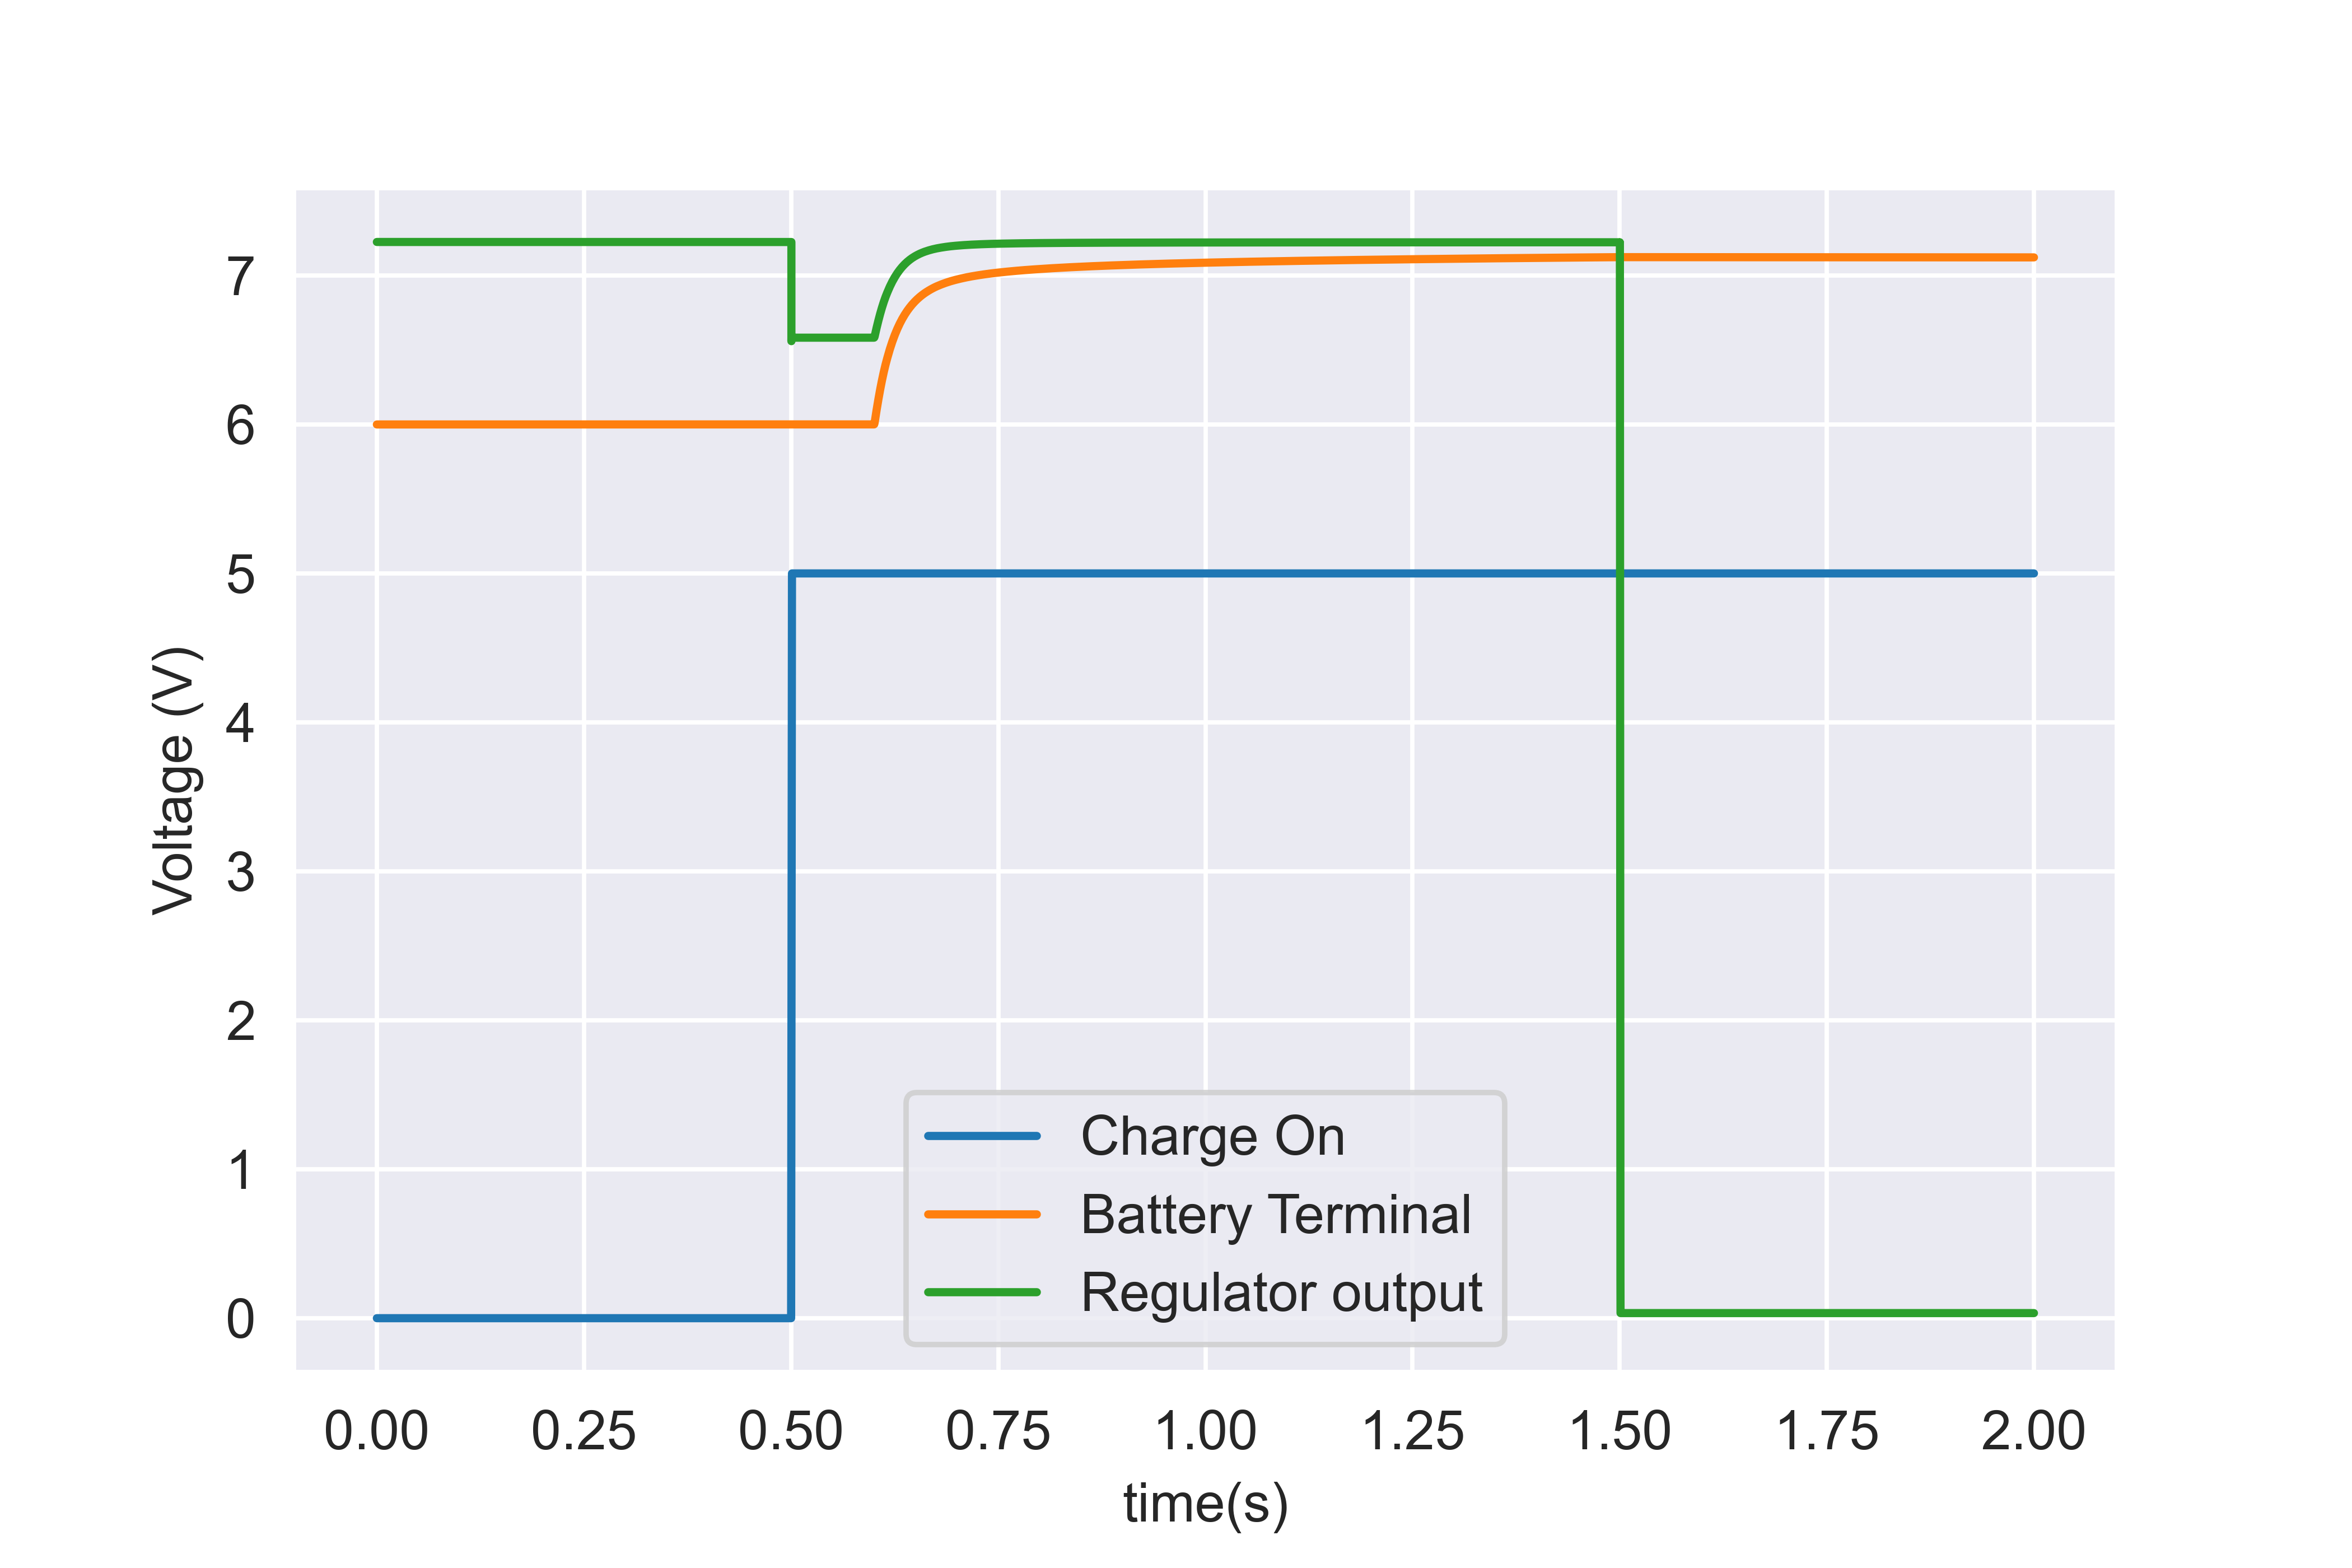
\includegraphics[width=1\linewidth]{./Figures/A2-1.png}
		    \caption{} \label{subfig:A2-1}
     \end{subfigure}
     \begin{subfigure}[]{0.42\textwidth}
             \centering
  		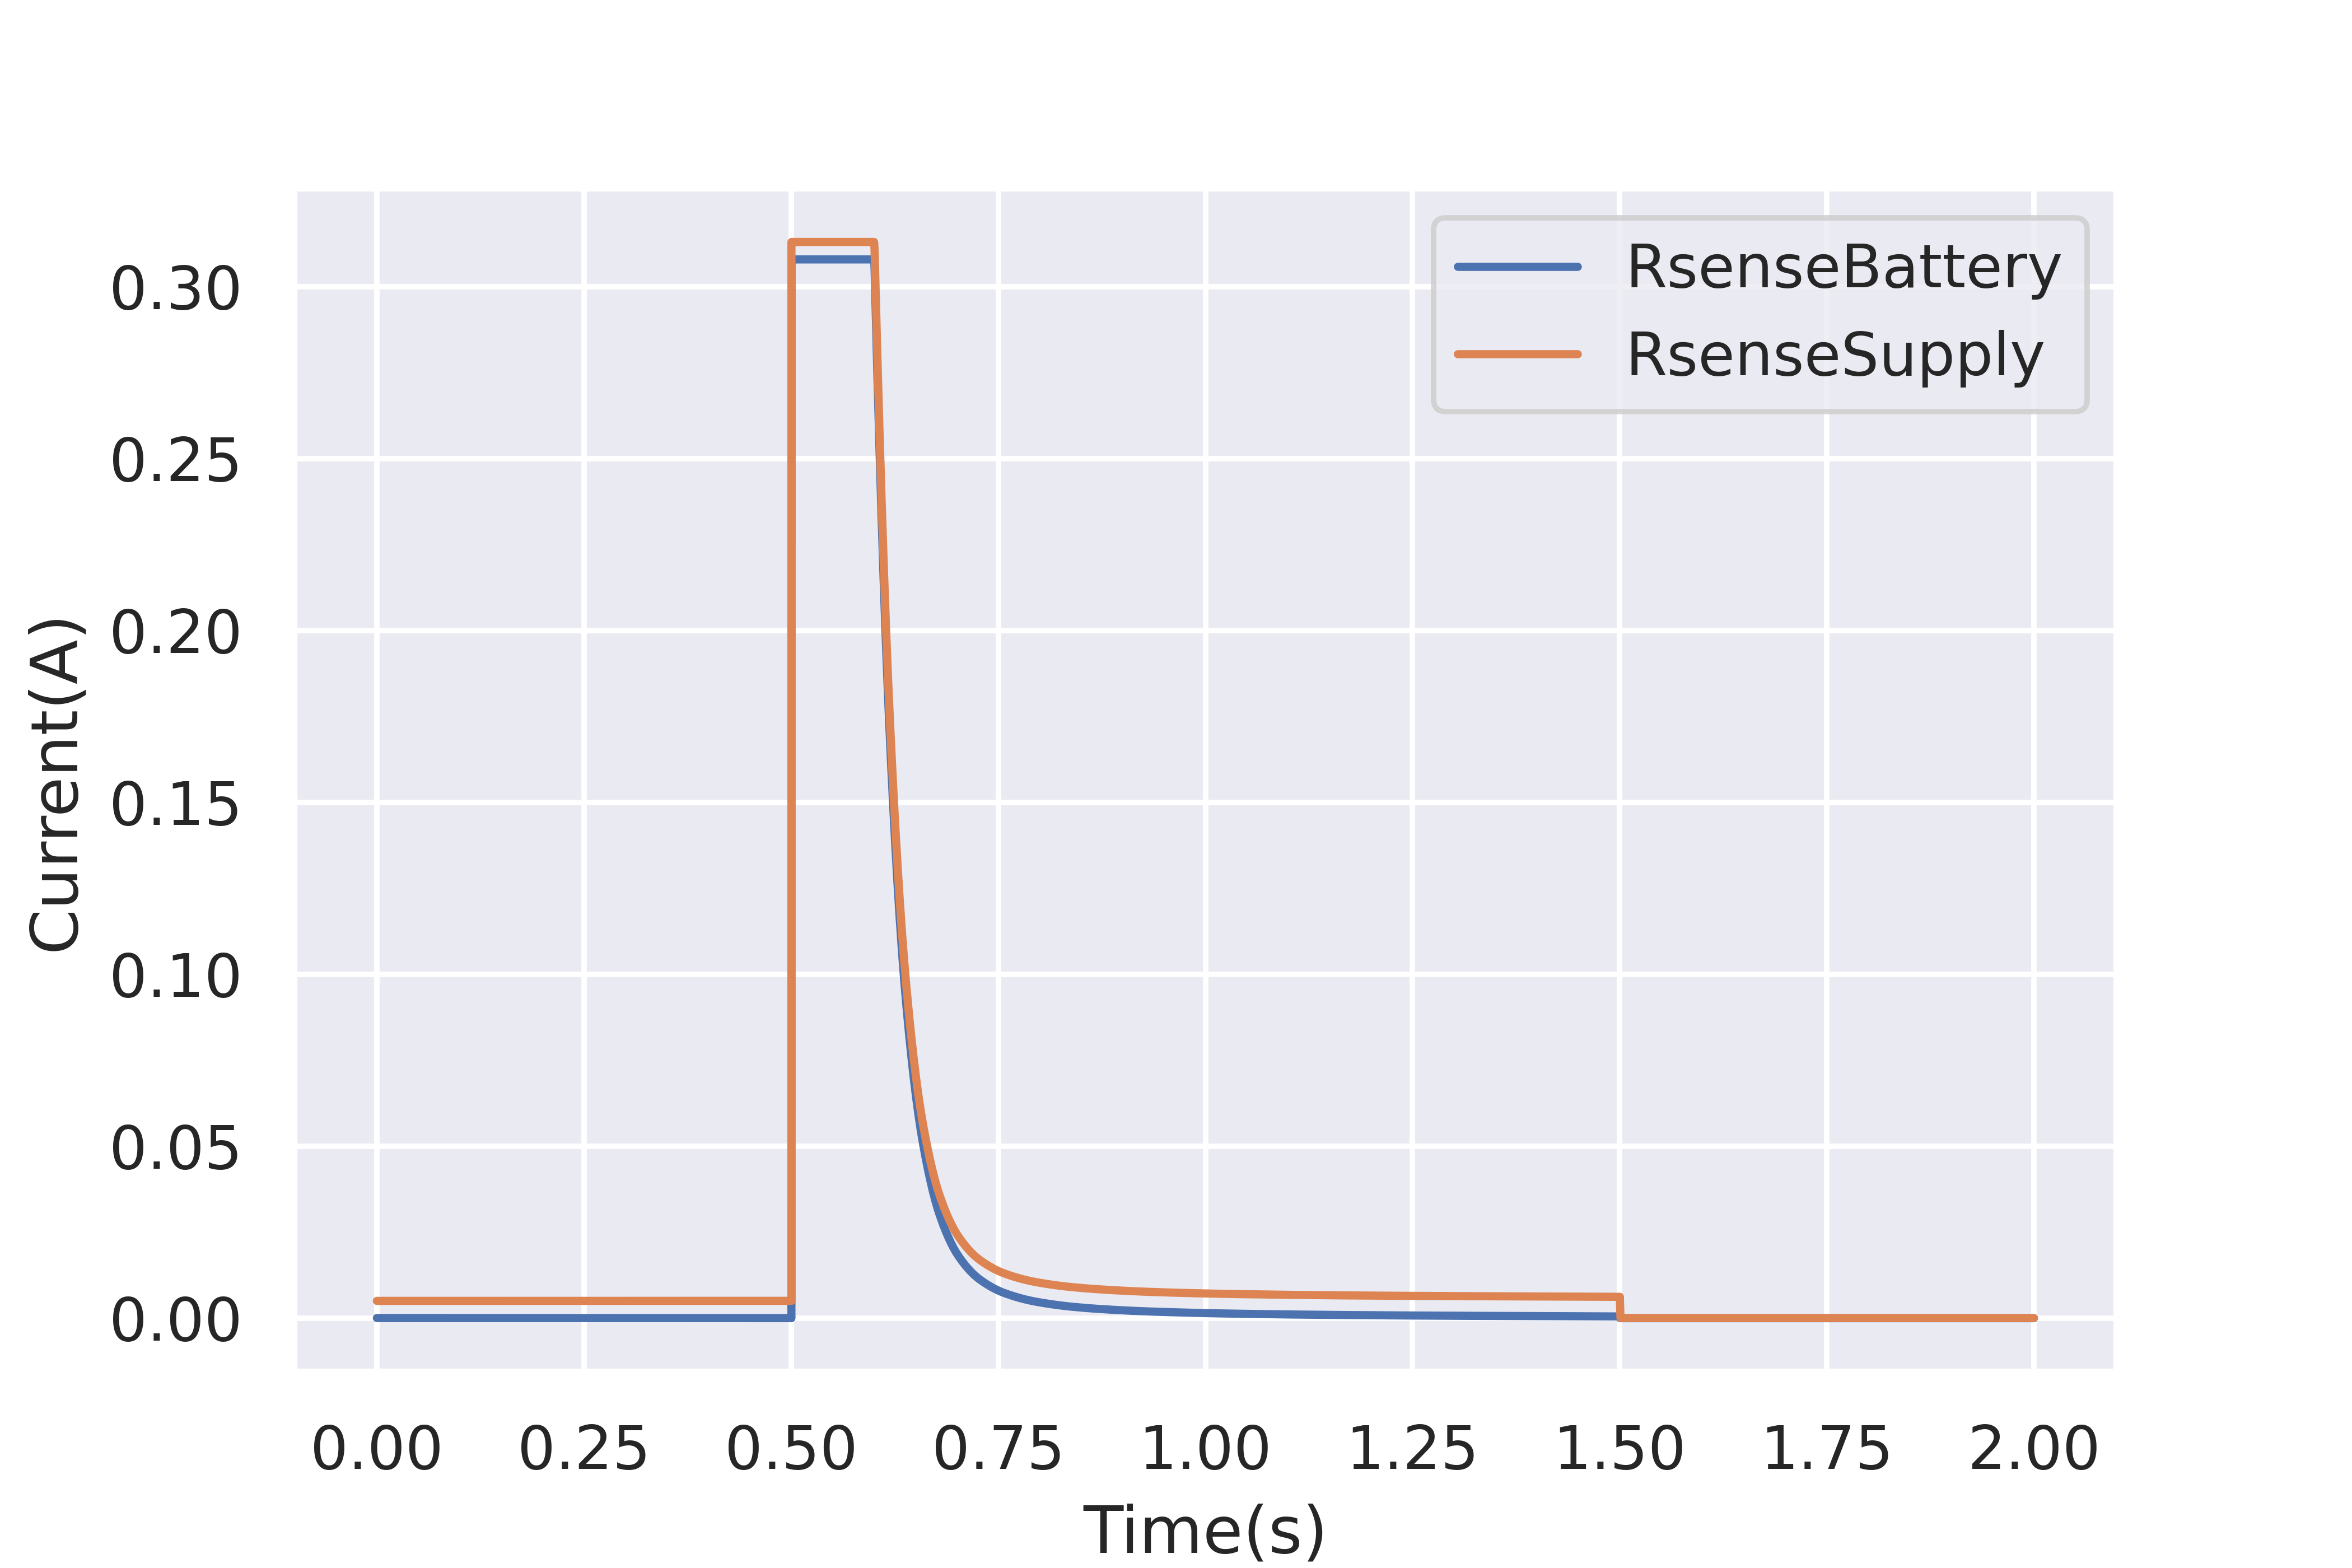
\includegraphics[width=1\linewidth]{./Figures/A2-2.png}
		   \caption{ } \label{subfig:A2-2}
     \end{subfigure}
   \caption[{LTSPICE switch turning on results}]{LTSpice Results for switch turning on  (a)  Relevant Voltages (b)  Relevant currents  }
    \label{fig:spiceReg}
 \end{figure}

 From figures \ref{subfig:A2-2} it can be seen that the maximum current flowing into the battery is just over 300mA. This current is much less than 1.2A and will therefore not damage the battery. The current only starts flowing when "charge on" (the control signal to the high side switch) goes high.
 
 \begin{figure}[!htb]
 \footnotesize
 \centering
    \begin{subfigure}[]{0.42\textwidth}
              \centering
  		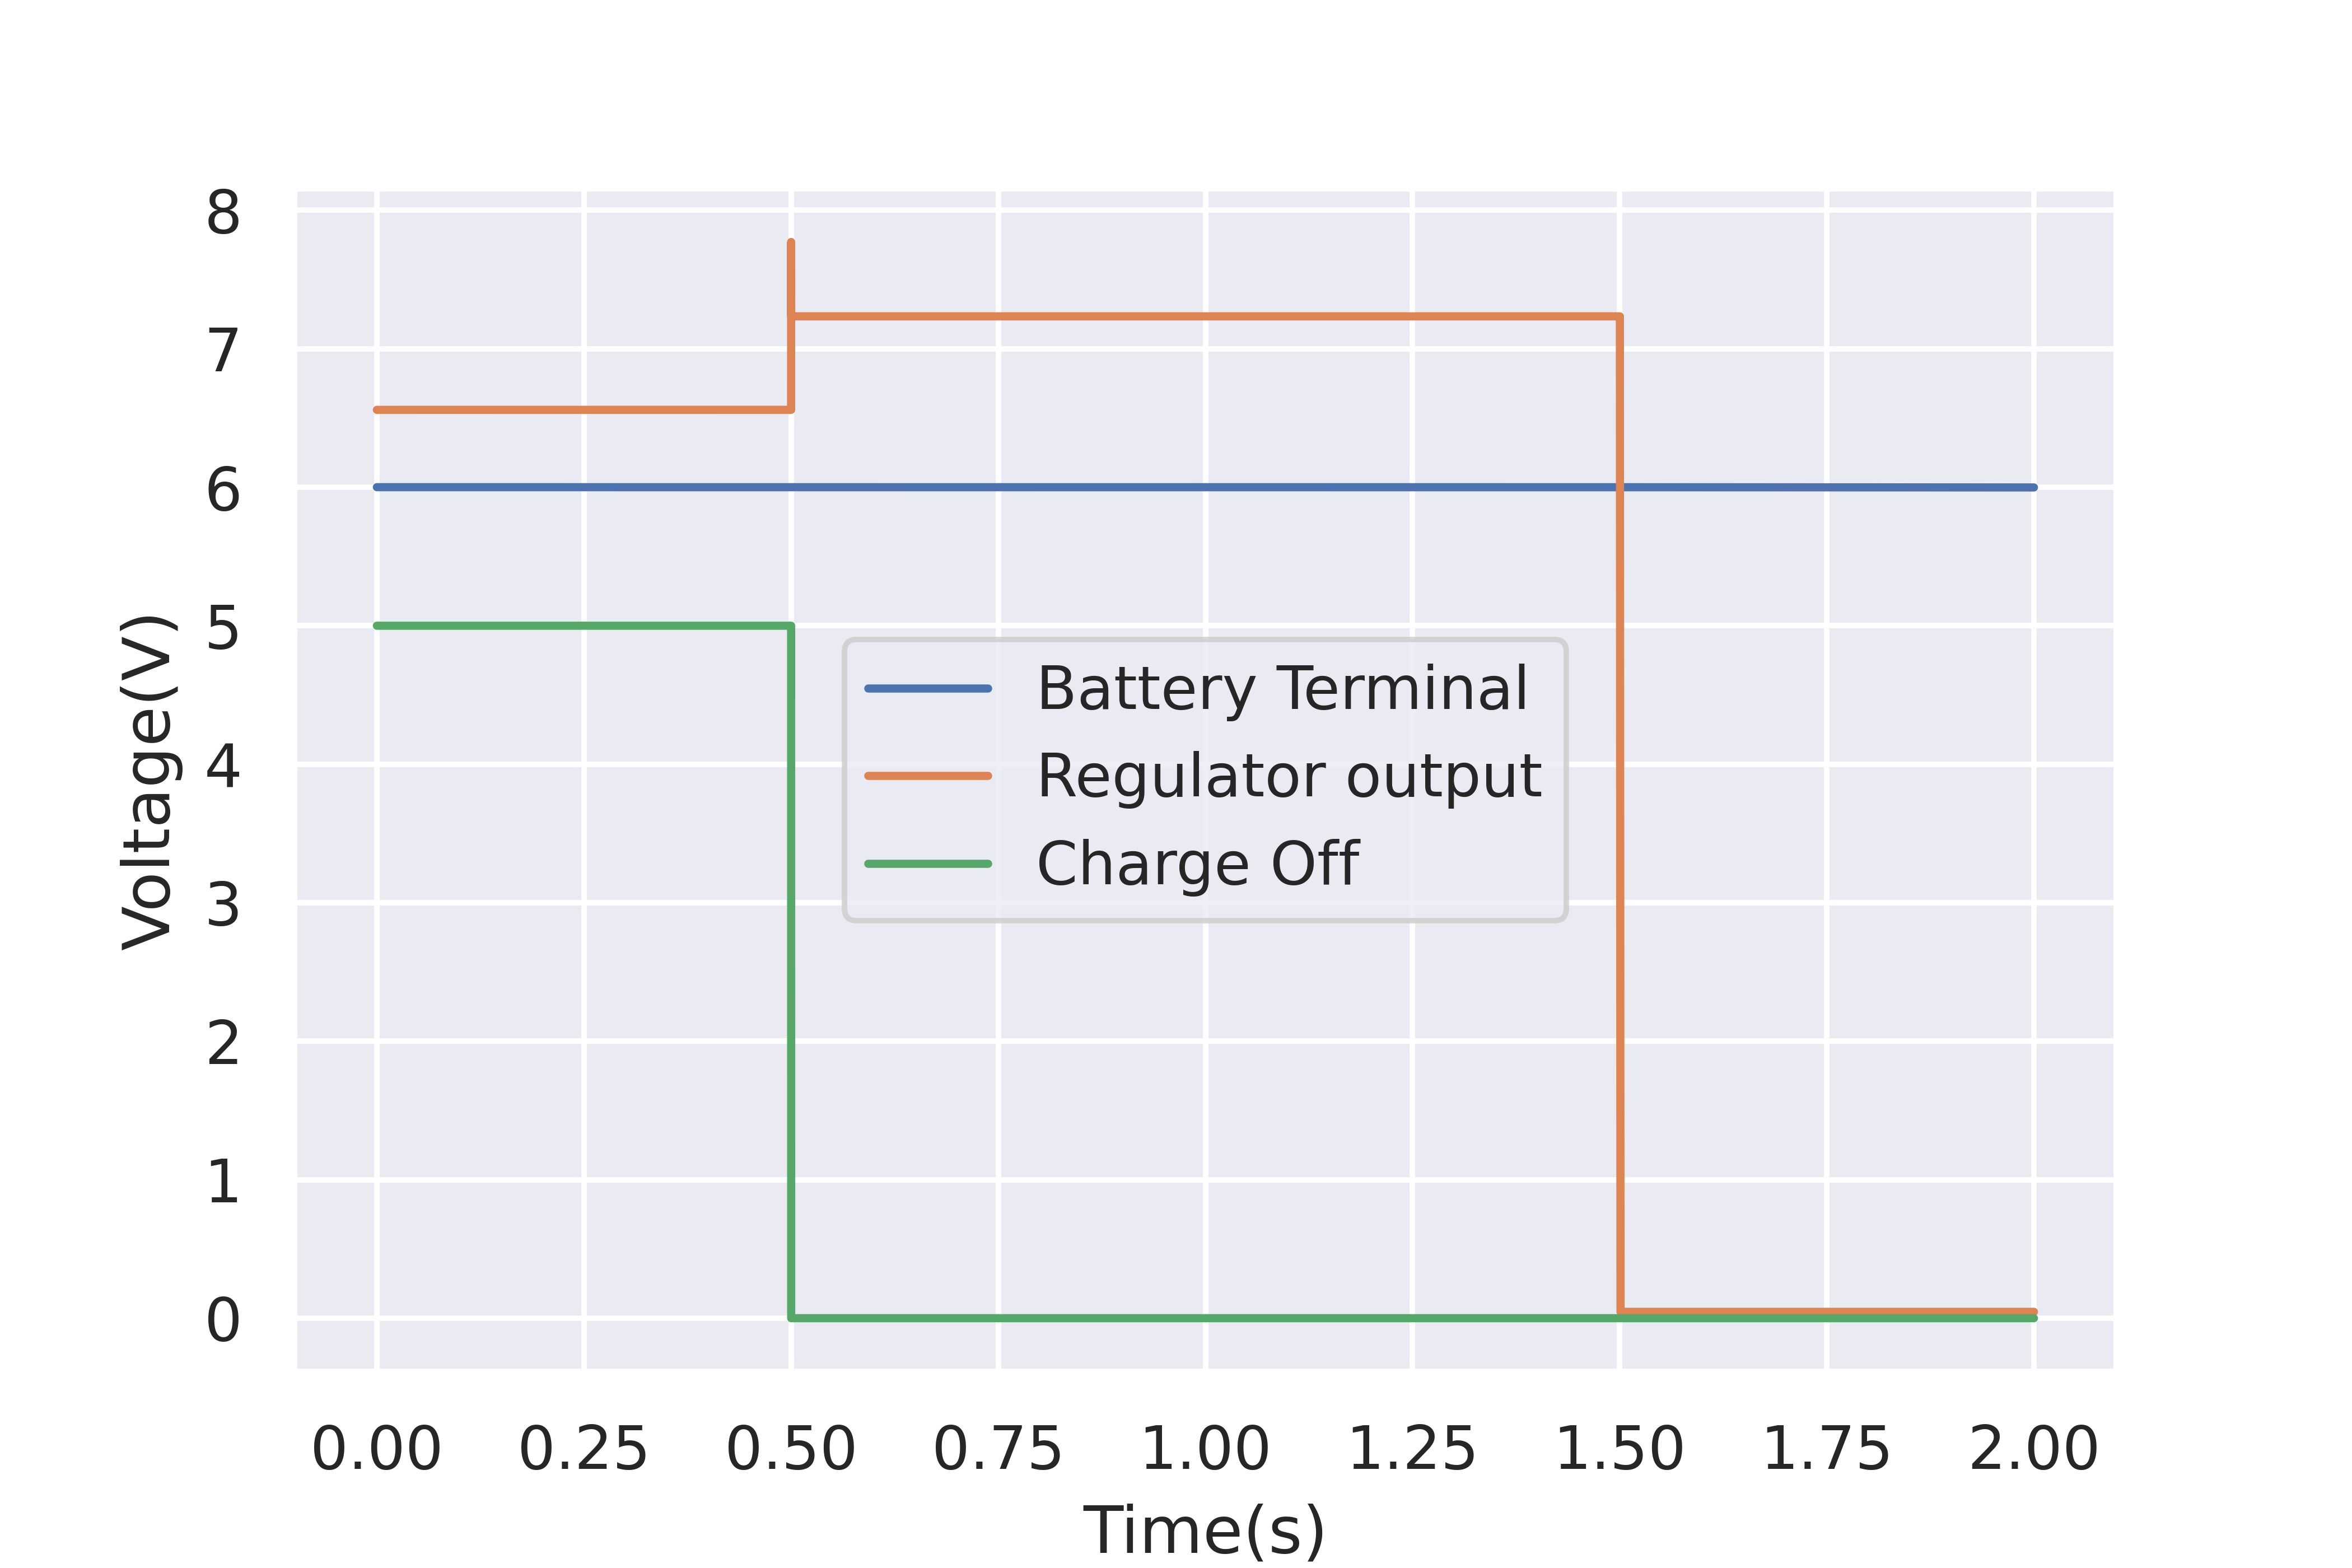
\includegraphics[width=1\linewidth]{./Figures/A2-3.png}
		    \caption{} \label{subfig:A2-3}
     \end{subfigure}
     \begin{subfigure}[]{0.42\textwidth}
             \centering
  		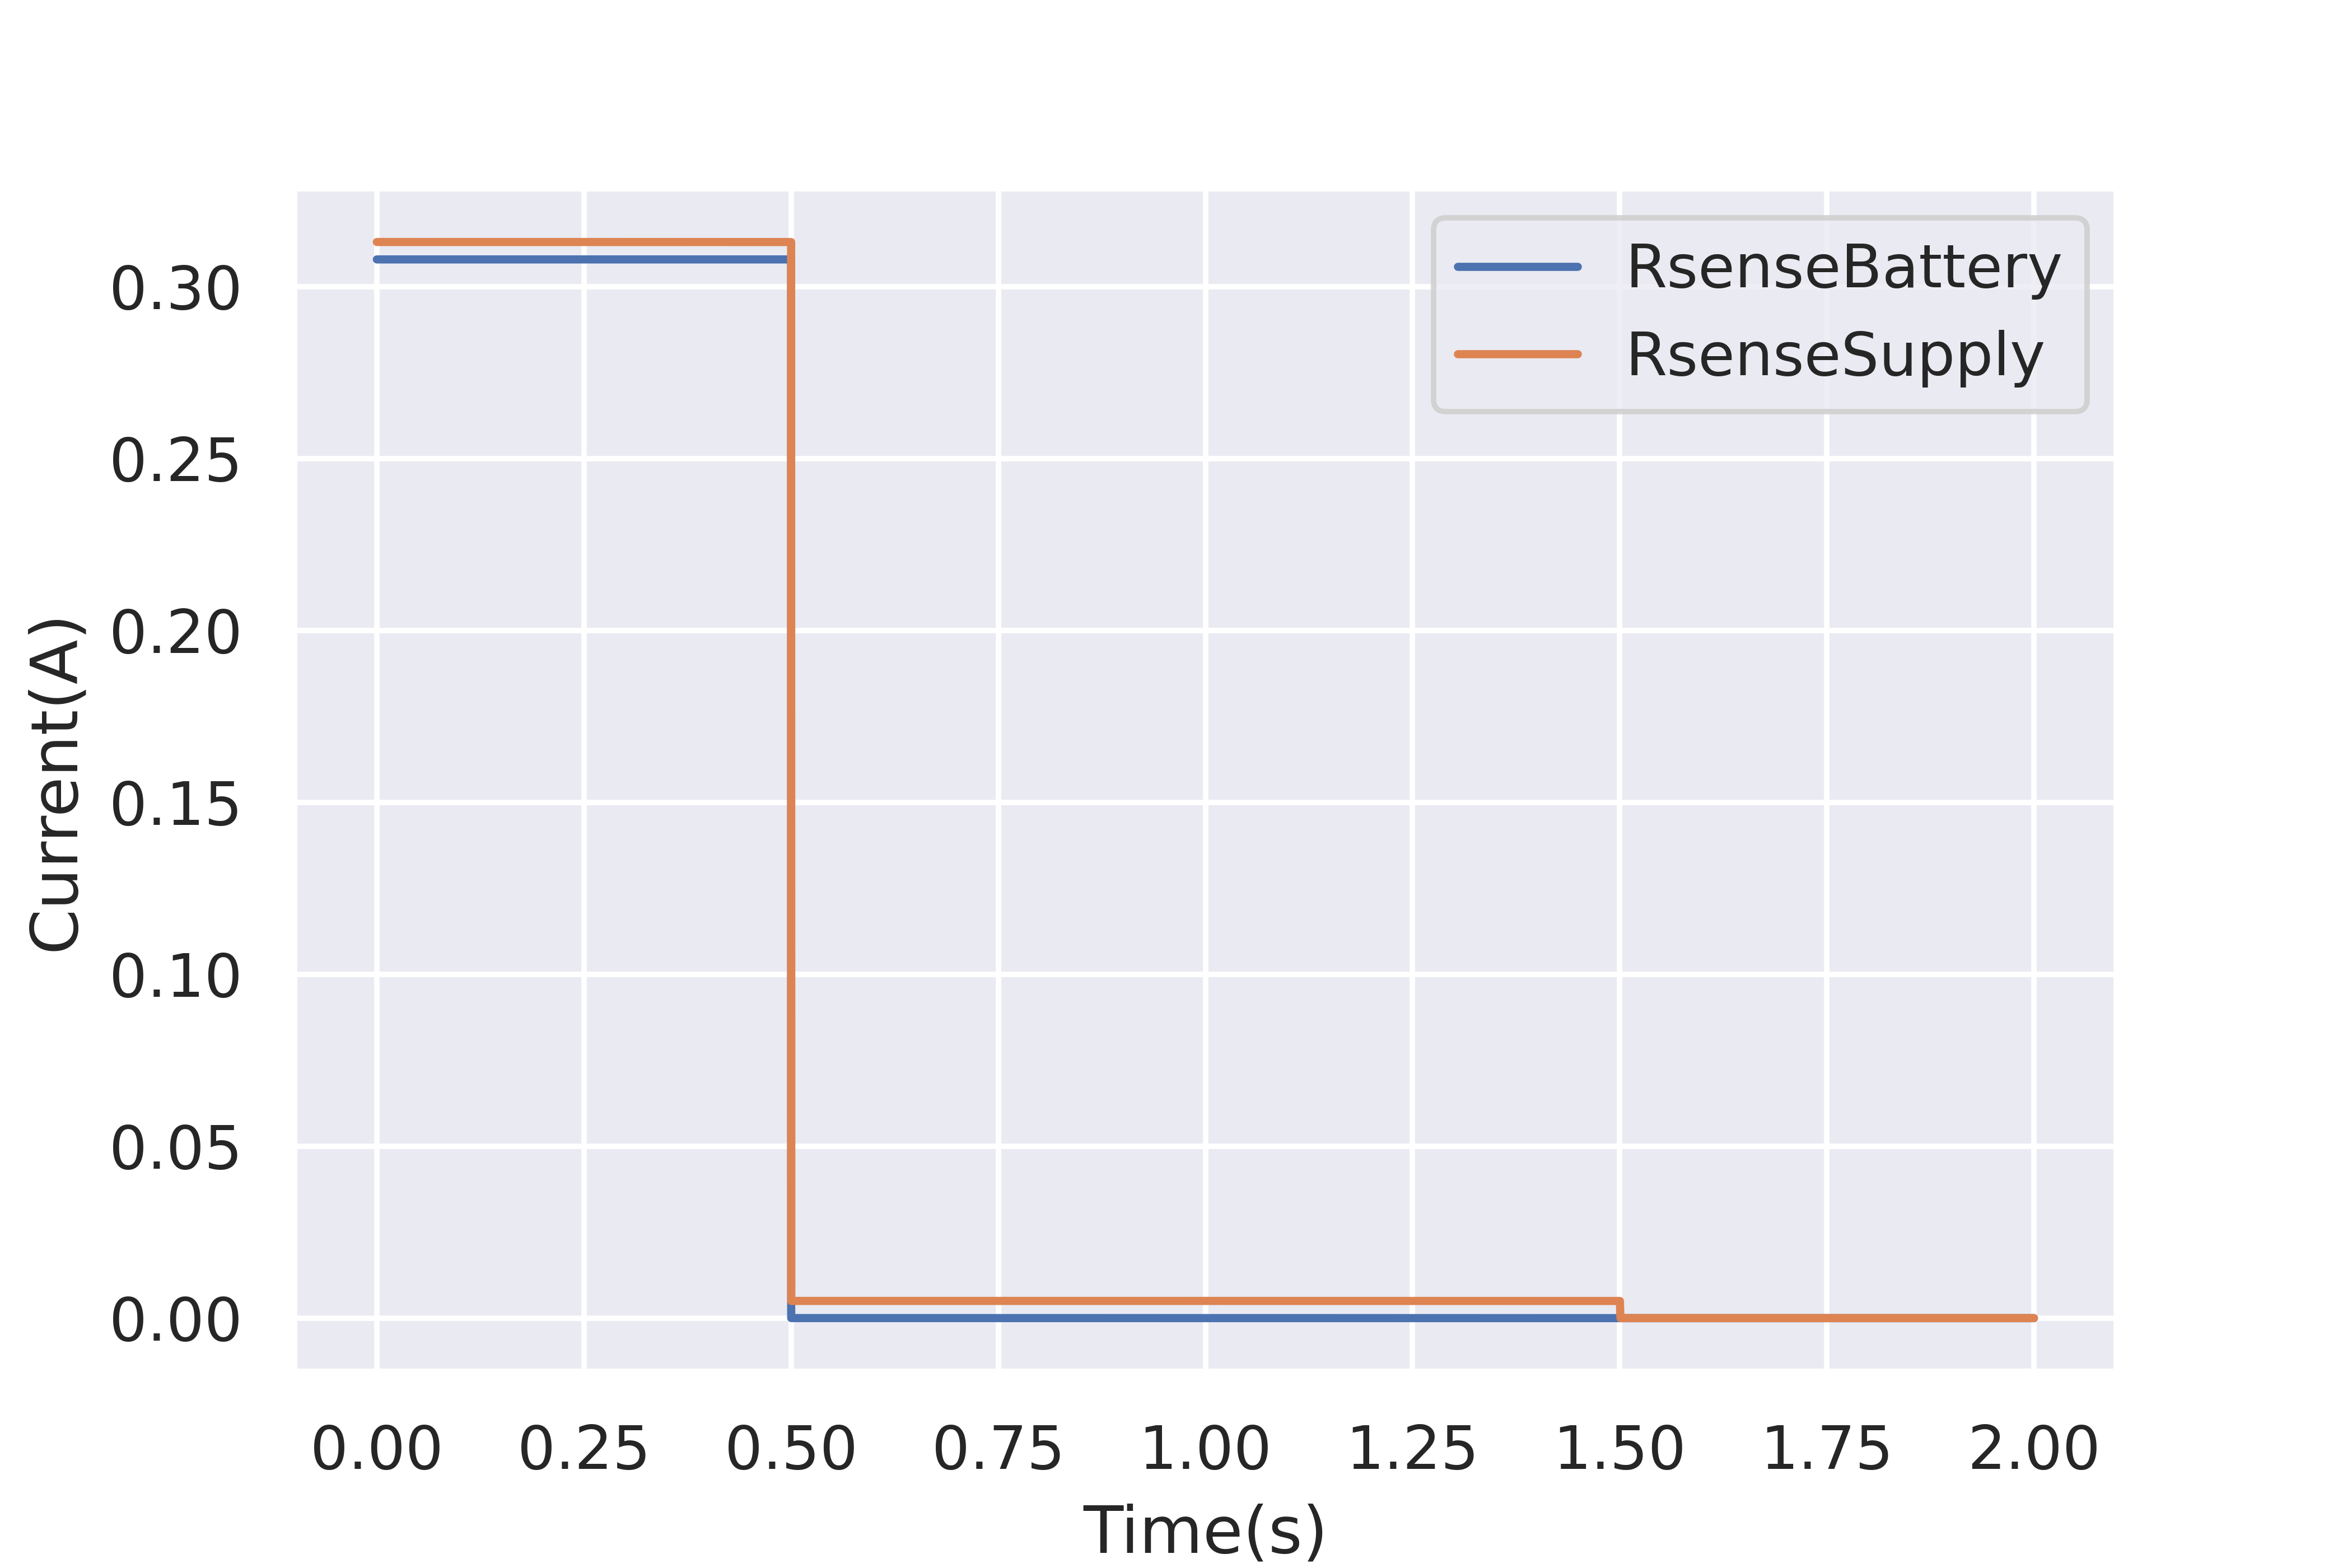
\includegraphics[width=1\linewidth]{./Figures/A2-4.png}
		   \caption{ } \label{subfig:A2-4}
     \end{subfigure}
   \caption[{LTSPICE switch turning off results}]{LTSpice Results for switch turning off  (a)  Relevant Voltages (b)  Relevant currents  }
    \label{fig:two}
 \end{figure}
 \newpage
 In figure \ref{fig:two} it can be seen that as soon as Charge Off goes low (NMOS turns off) the current to the battery stops flowing and the battery voltage remains at 6V.



 \begin{figure}[!htb]
 \footnotesize
 \centering
    \begin{subfigure}[]{0.42\textwidth}
              \centering
  		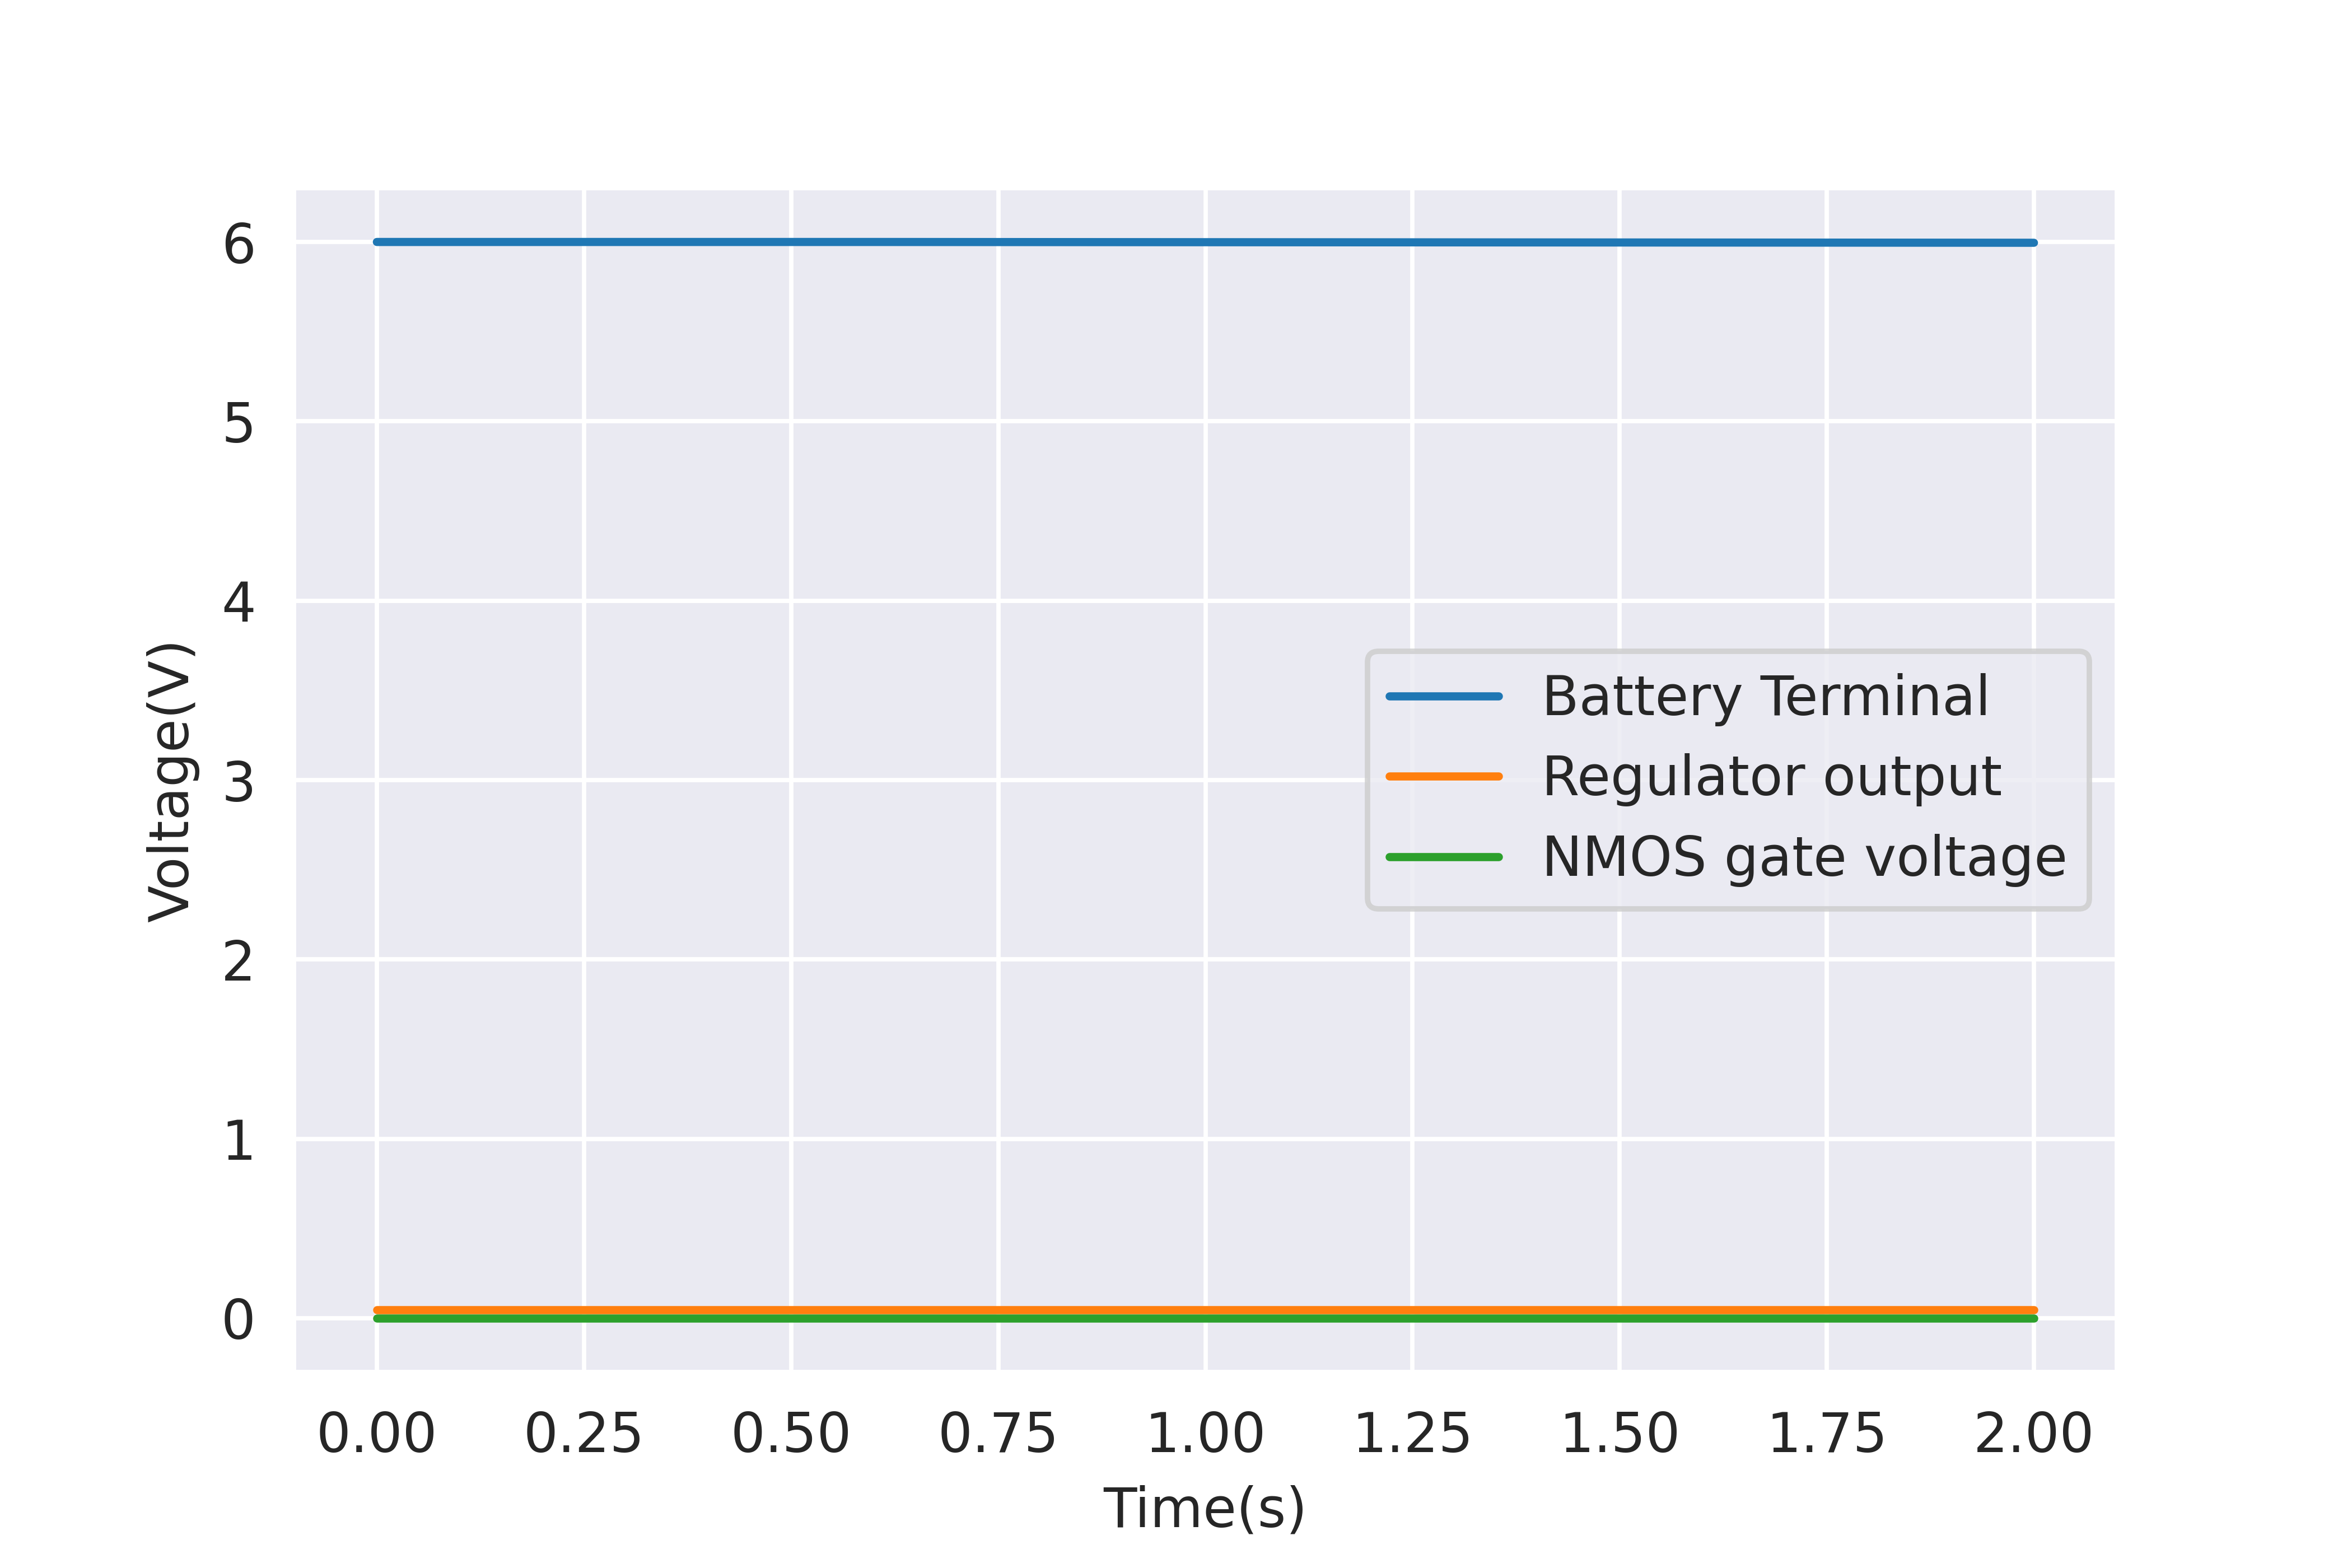
\includegraphics[width=1\linewidth]{./Figures/A2-5.png}
		    \caption{} \label{subfig:A2-5}
     \end{subfigure}
     \begin{subfigure}[]{0.42\textwidth}
             \centering
  		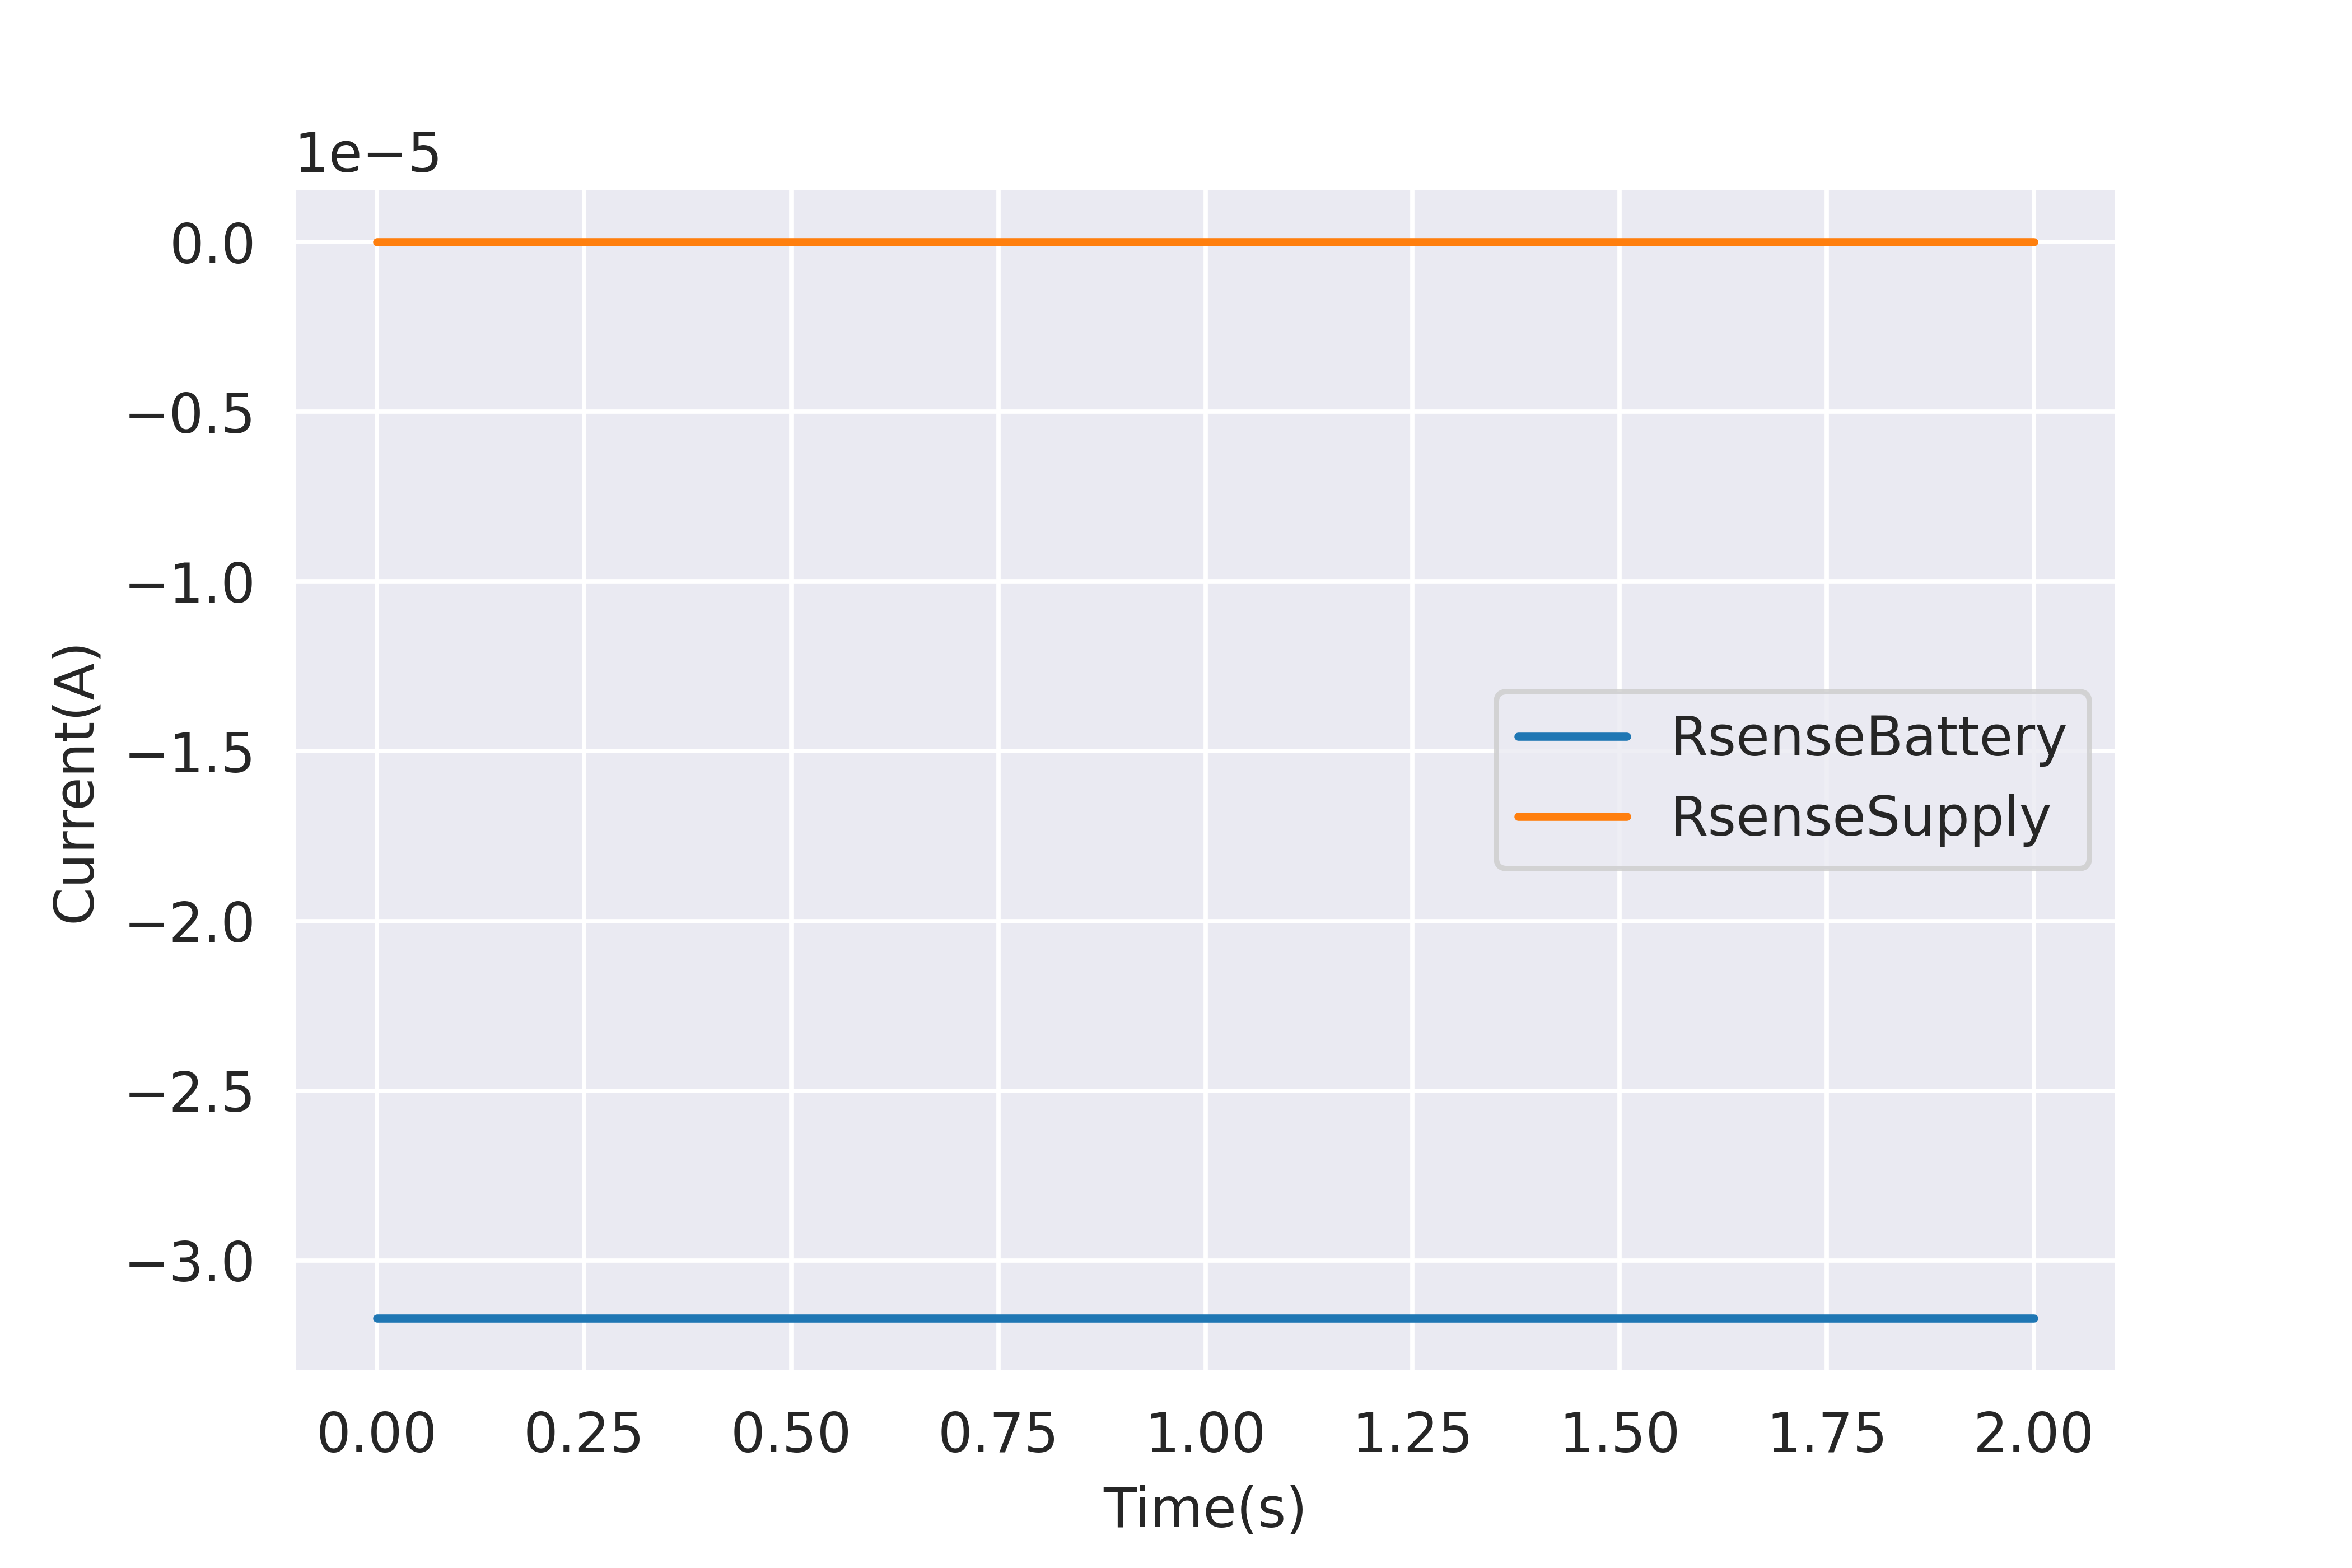
\includegraphics[width=1\linewidth]{./Figures/A2-6.png}
		   \caption{ } \label{subfig:A2-6}
     \end{subfigure}
   \caption[{LTSPICE switch off and supply off results}]{LTSpice Results for supply off and NMOS gate pulled low  (a)  Relevant Voltages (b)  Relevant currents  }
    \label{fig:three}
 \end{figure}
In figure \ref{fig:three} both the supply and the switch are off. This then shows the discharge current of just above 30\textmu A. It is small enough that I would say specifications are met.


%**********************************************

\begin{table}[!htb]
        \centering
        \footnotesize
        \caption{Measured Values}
         \begin{tabular}{lrrrr}
          \toprule
             & Voltage at battery connection terminal \\
             &  [V] \\
          \midrule
          Open Circuit & 7.27     \\
          1K Load &  7.1     \\
          10K load &  7.0     \\

          \bottomrule
        \end{tabular}
     \label{tab:regmeas}
\end{table}
From table \ref{tab:regmeas} it can be seen that voltage is operating in the correct region of less than 7.2V. More results regarding the charging can be found in section \ref{sec:sysRes} in table \ref{tab:batsys}.



 

%**********************************************
%%%%%%%%%%%%%%%%%%%%%%%%%%%%%%%%%%%%%%%%%%%%%%%%%
\newpage
\section{High side switch on supply side}

\begin{figure}[!htb]
 \footnotesize
 \centering
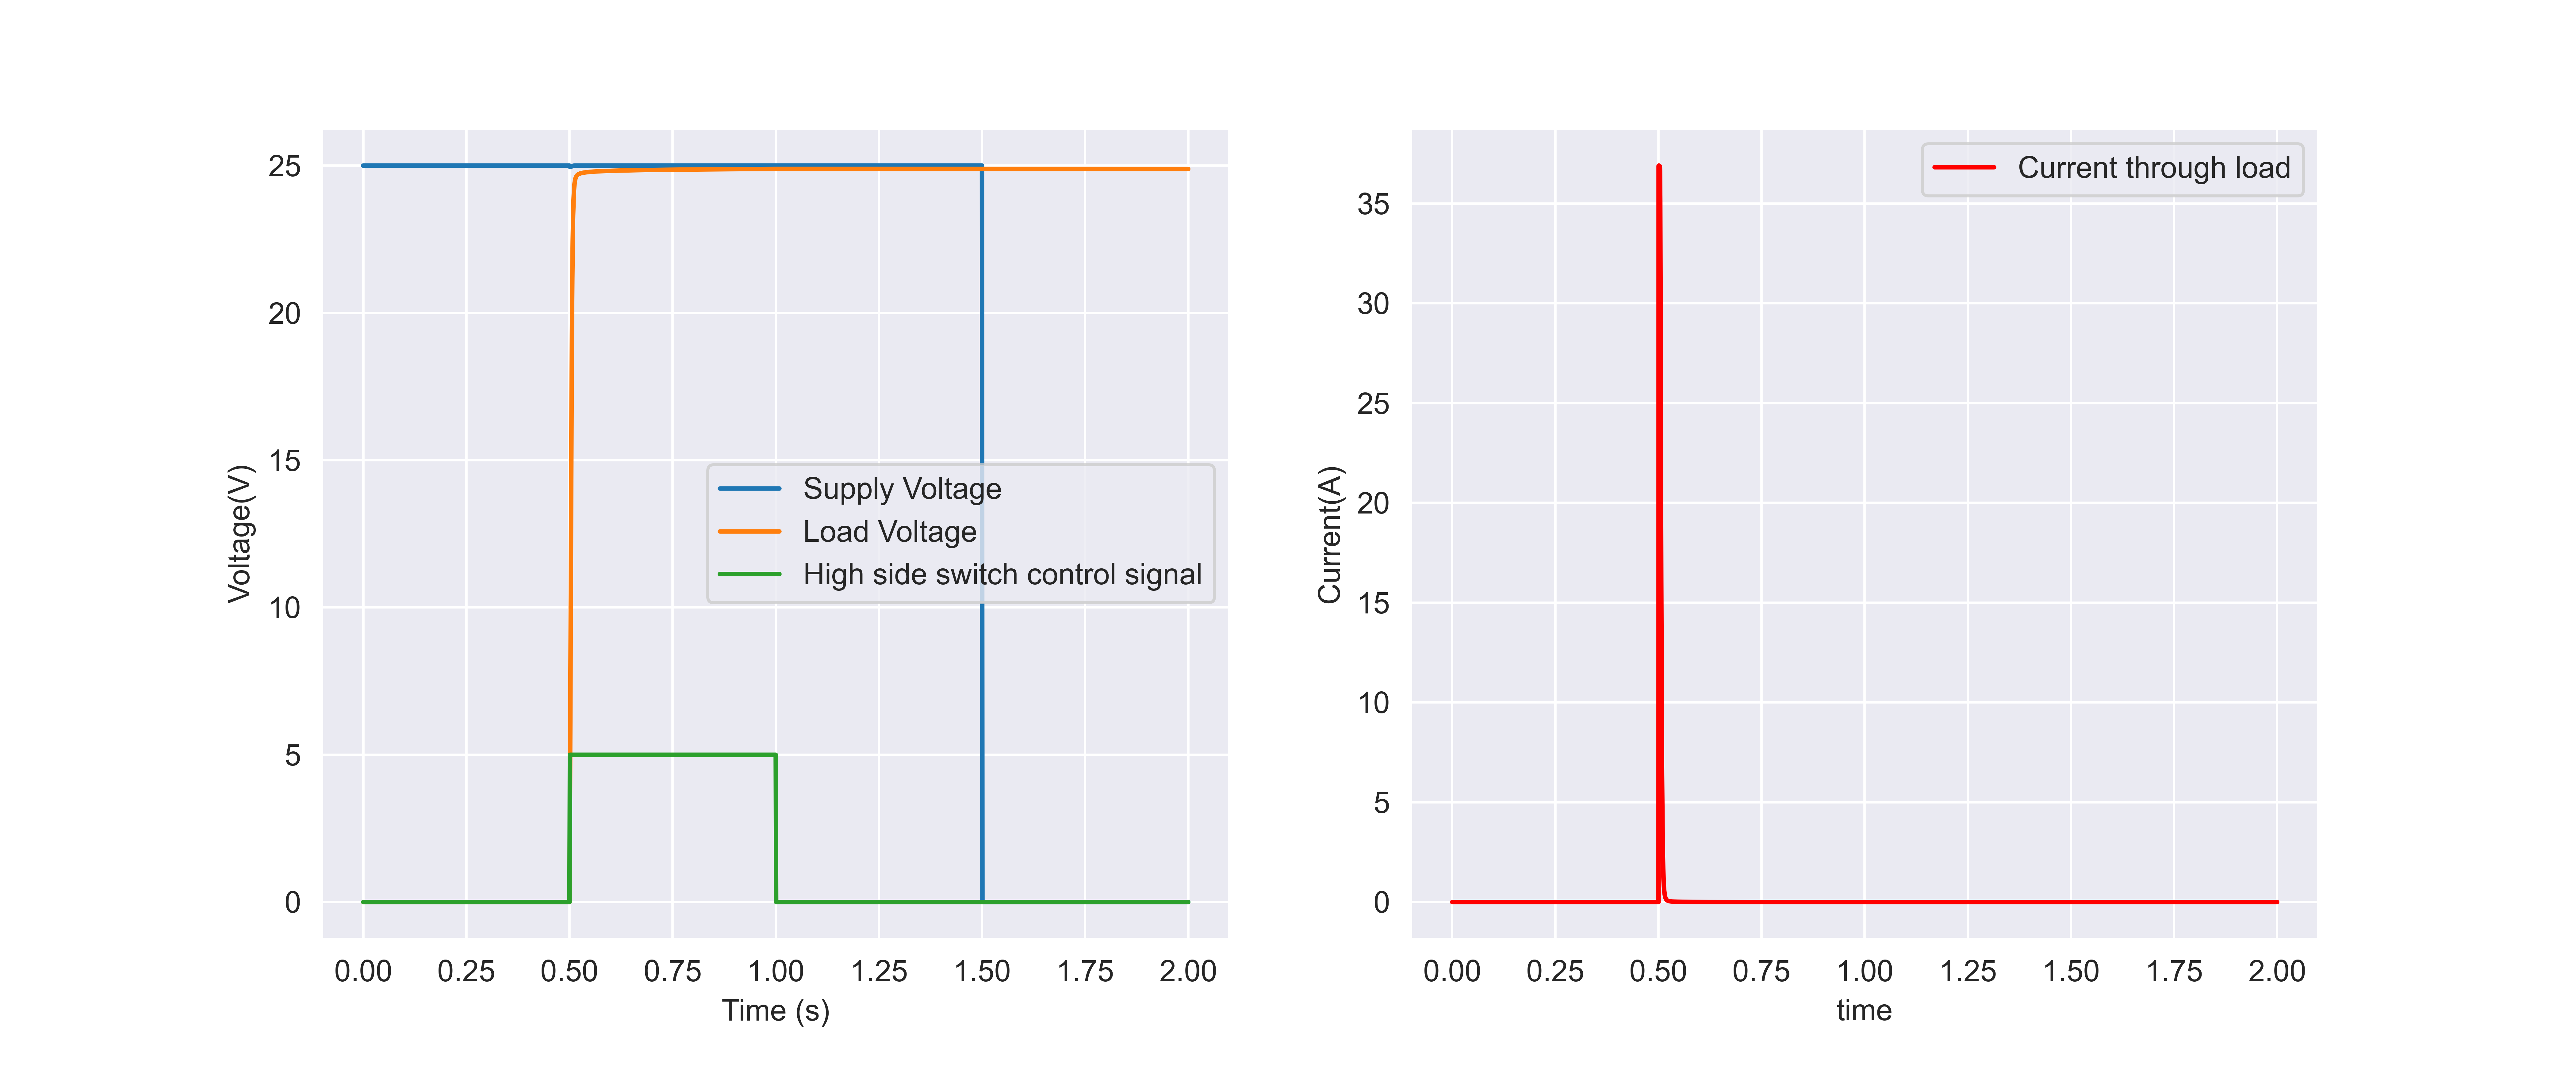
\includegraphics[width=0.8\textwidth]{Figures/A1.png}
\caption{LTSpice simulation results for high side switch on the supply side}
\label{fig:high-res}
 \end{figure}
 
 From figure \ref{fig:high-res} it can be seen that as soon as the high side witch control signal goes high, the load voltage changes to approximately the supply voltage. The current spikes as seen because the capacitor at the load charges up to the supply voltage very quickly.

\begin{table}[!htb]
        \centering
        \footnotesize
        \caption{Highside switch measurements}
         \begin{tabular}{lrrrr}
          \toprule
             & voltage from source to gate of the PMOS \\
             &  [V] \\
          \midrule
          Control signal at NMOS gate high &     6.94\\
          Control signal at NMOS gate low  &   0\\
         

          \bottomrule
        \end{tabular}
     \label{tab:PMOSmeas}
\end{table}
From the values in table \ref{tab:PMOSmeas} it can be seen that when the NMOS gate voltage goes high a voltage above the threshold voltage of the PMOS is applied, thus turning the switch on. For additional proof that the switch works, refer to figure \ref{fig:meas} where this switch successfully controlled the switching on and off of the charging circuit.
%%%%%%%%%%%%%%%%%%%%%%%%%%%%%%%%%%%%%%%%%%%%%%%%%
\newpage
\section{Undervoltage protection}
\begin{figure}[!htb]
 \footnotesize
 \centering
    \begin{subfigure}[]{0.45\textwidth}
              \centering
  		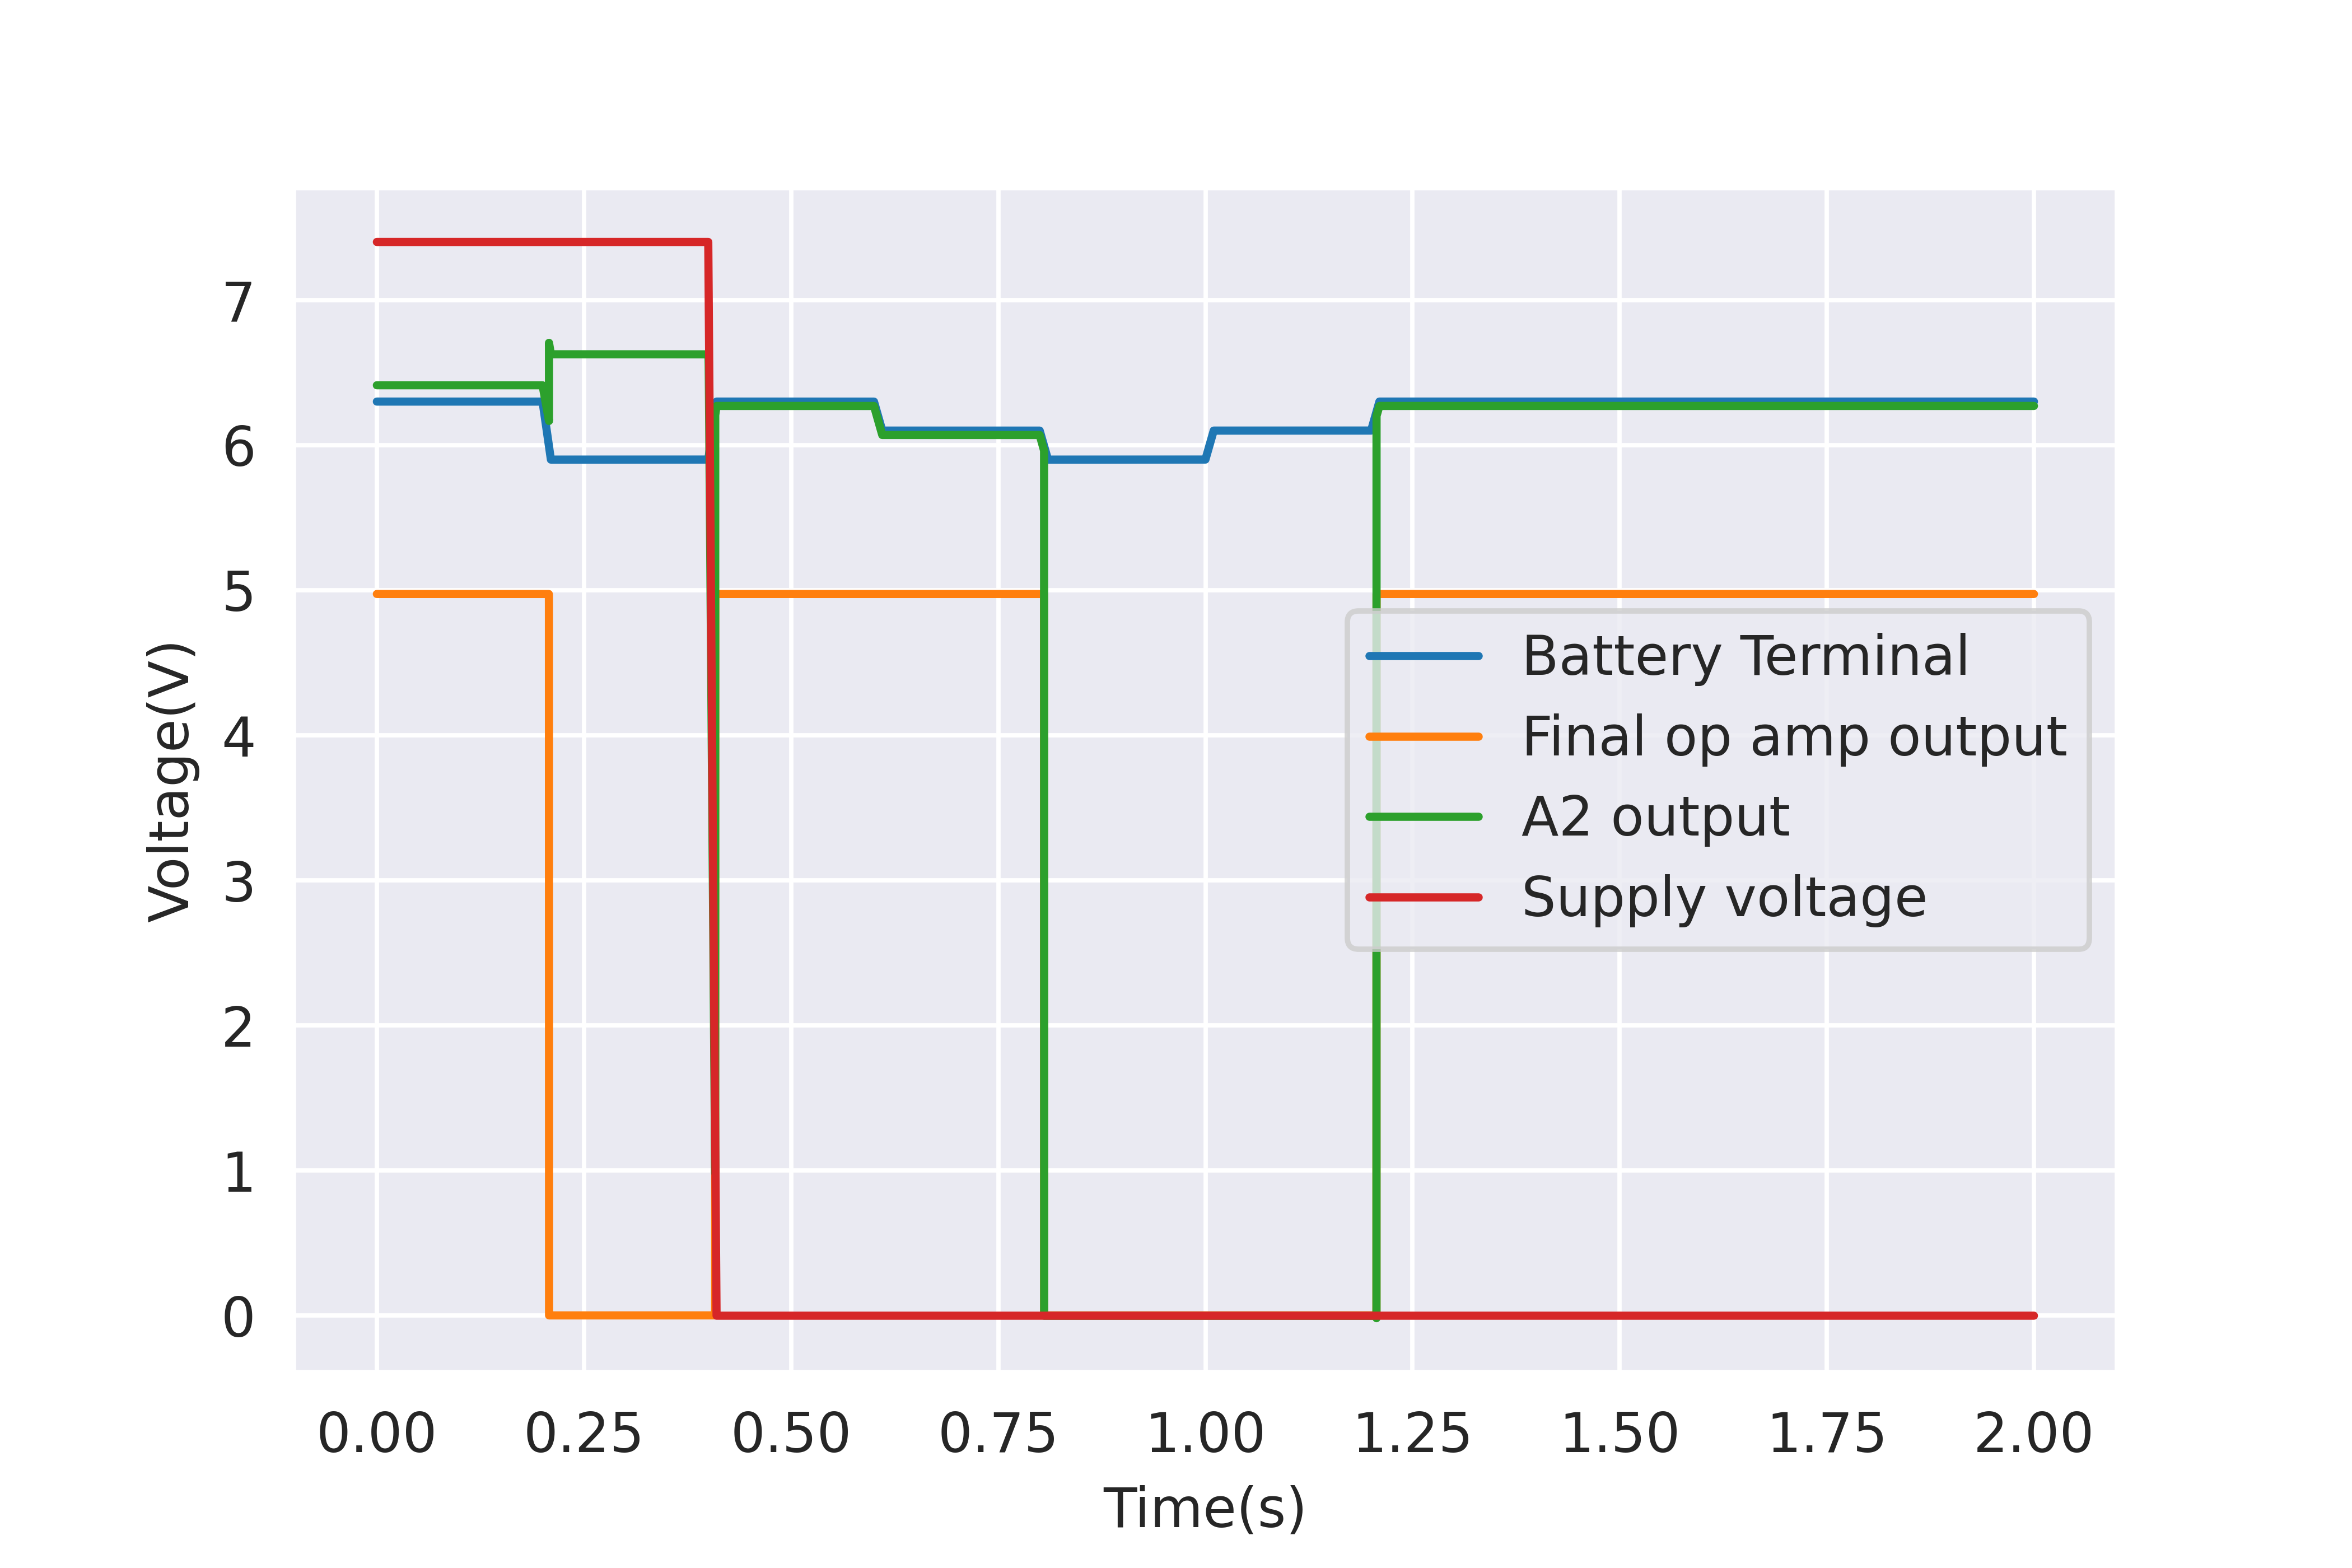
\includegraphics[width=1\linewidth]{./Figures/A31.png}
		    \caption{} \label{subfig:voltage}
     \end{subfigure}
     \begin{subfigure}[]{0.45\textwidth}
             \centering
  		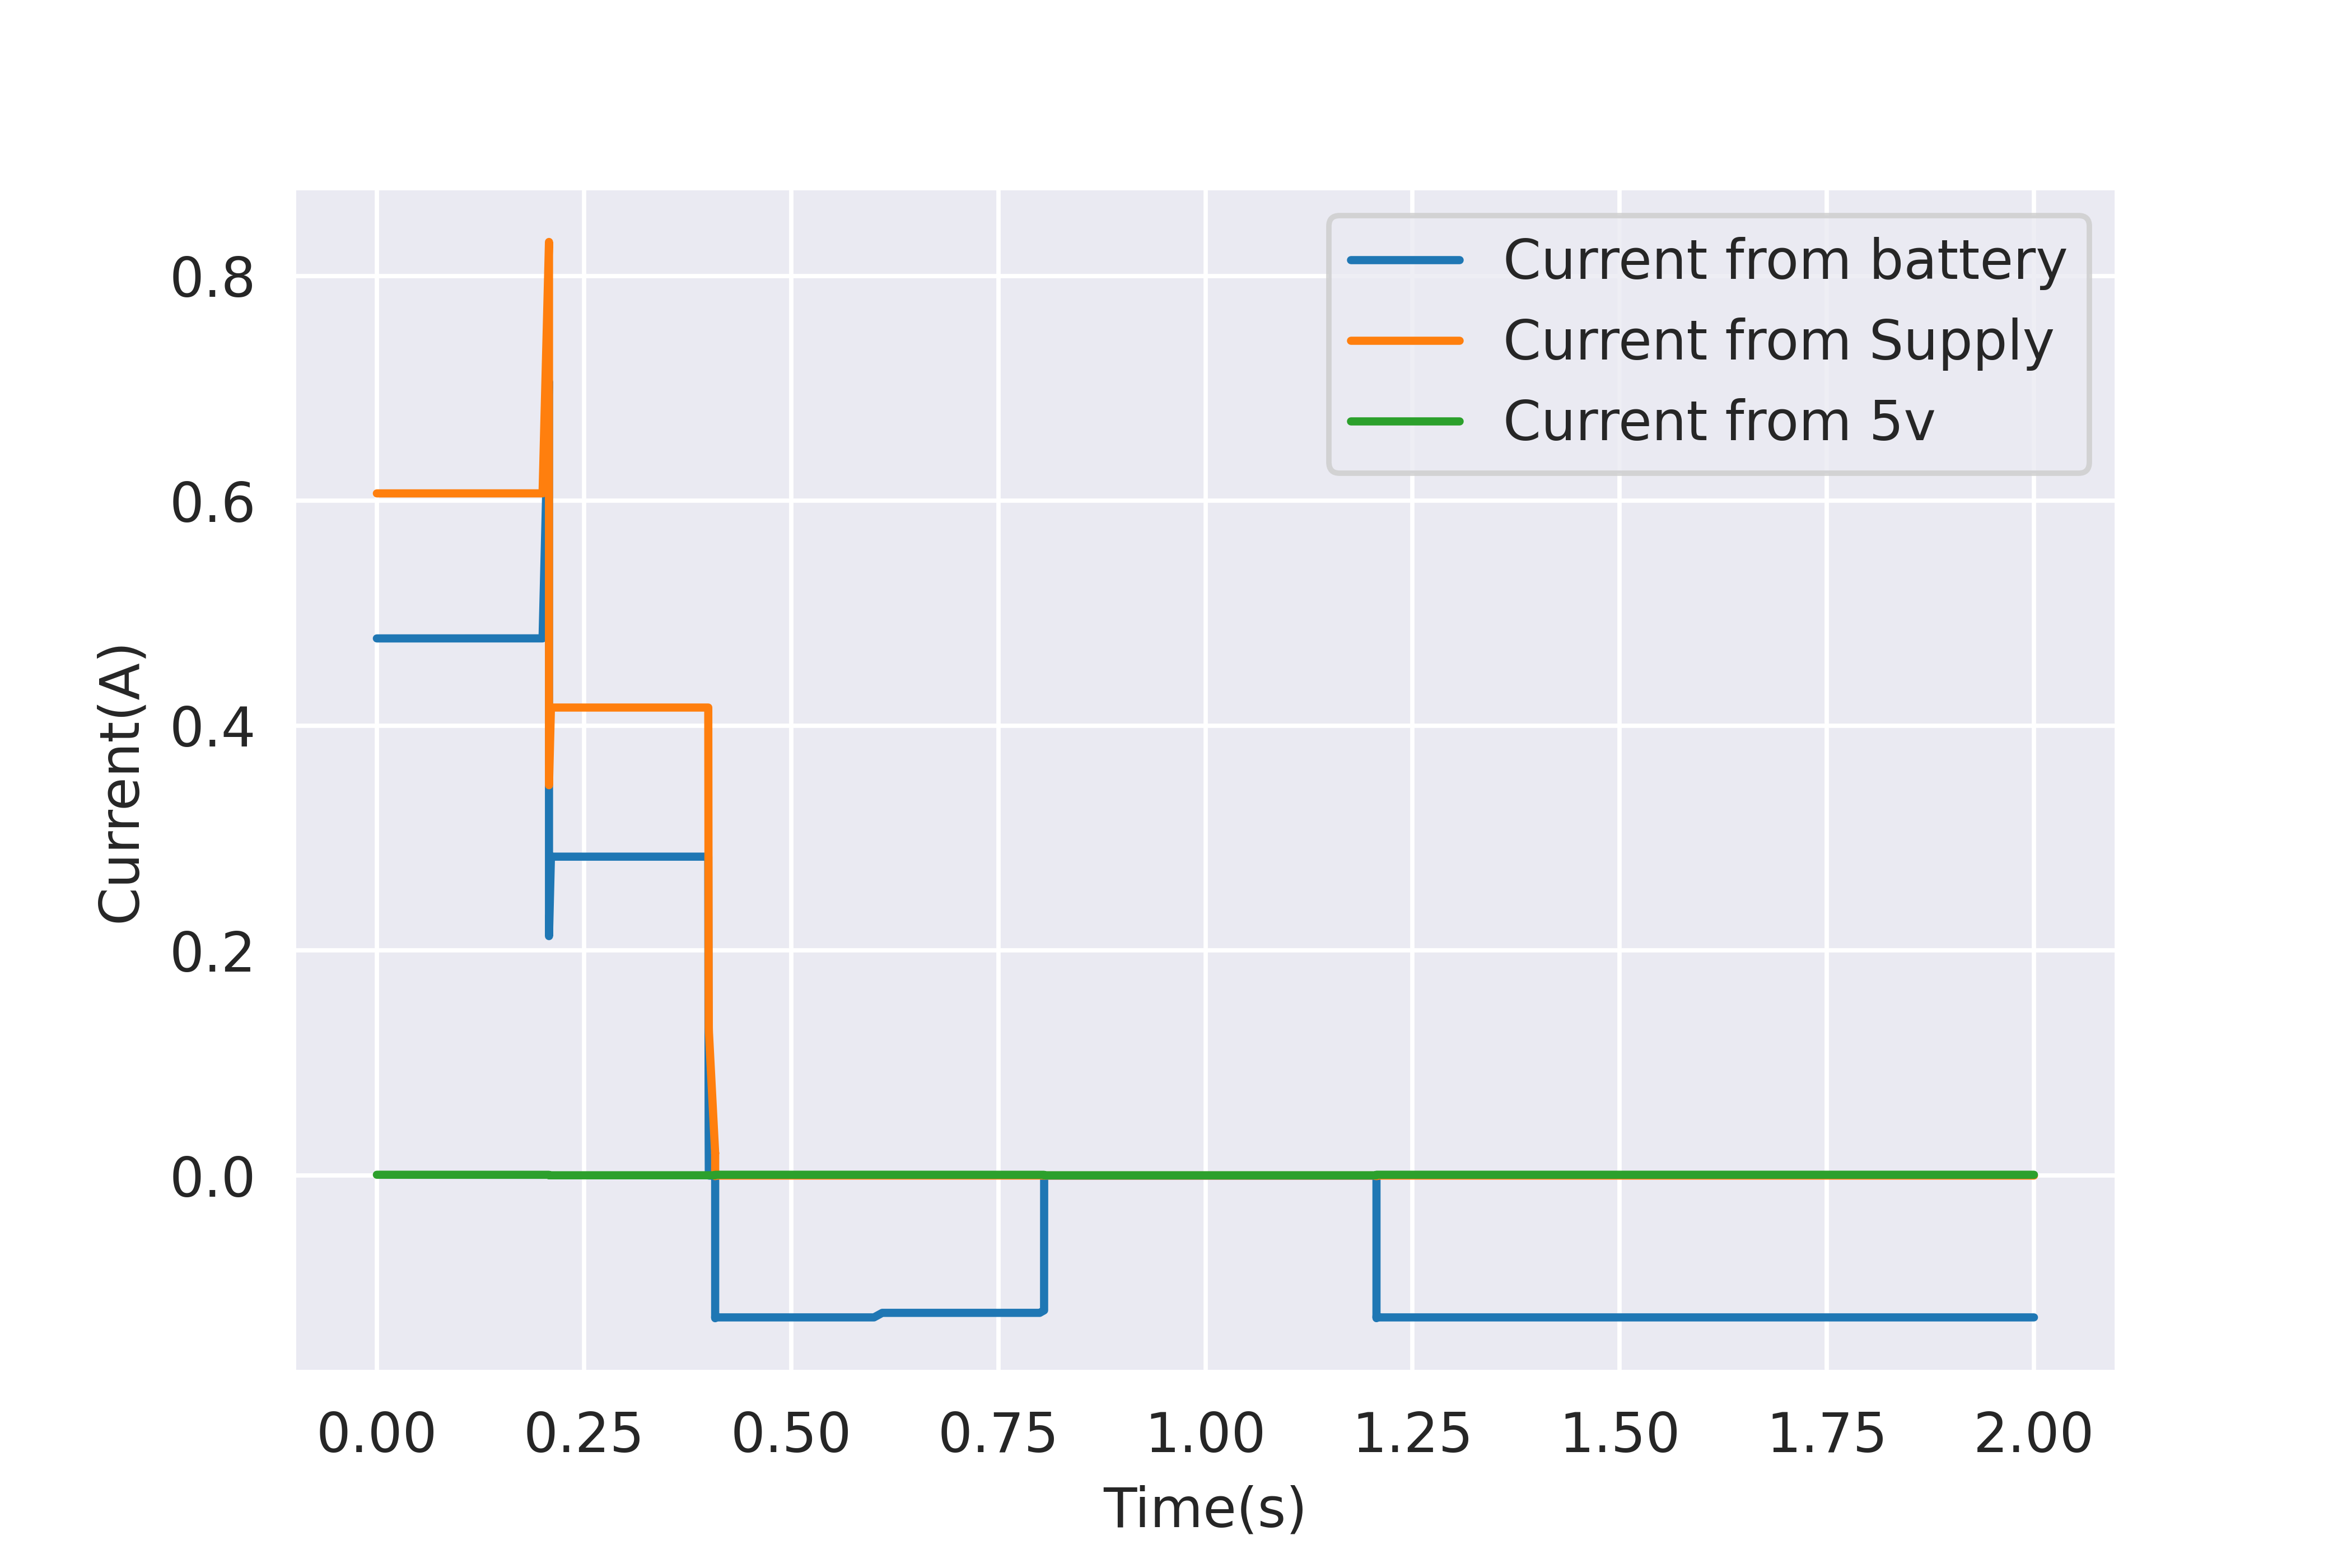
\includegraphics[width=1\linewidth]{./Figures/A32.png}
		   \caption{ } \label{subfig:current}
     \end{subfigure}
   \caption[{LT spice Results}]{LT spice results   (a) Relevant Voltages (b)  Relevant Currents }
    \label{fig:lt}
 \end{figure}


From figure \ref{subfig:voltage} it can be seen that the op amp transitions at the correct of 6V and 6.2V respectively. From figure \ref{subfig:current} it can be seen that the current out of the 5V regulator is less than 10mA and that the op amp output corresponds to the discharging from the battery. 


\begin{figure}[!htb]
\centering
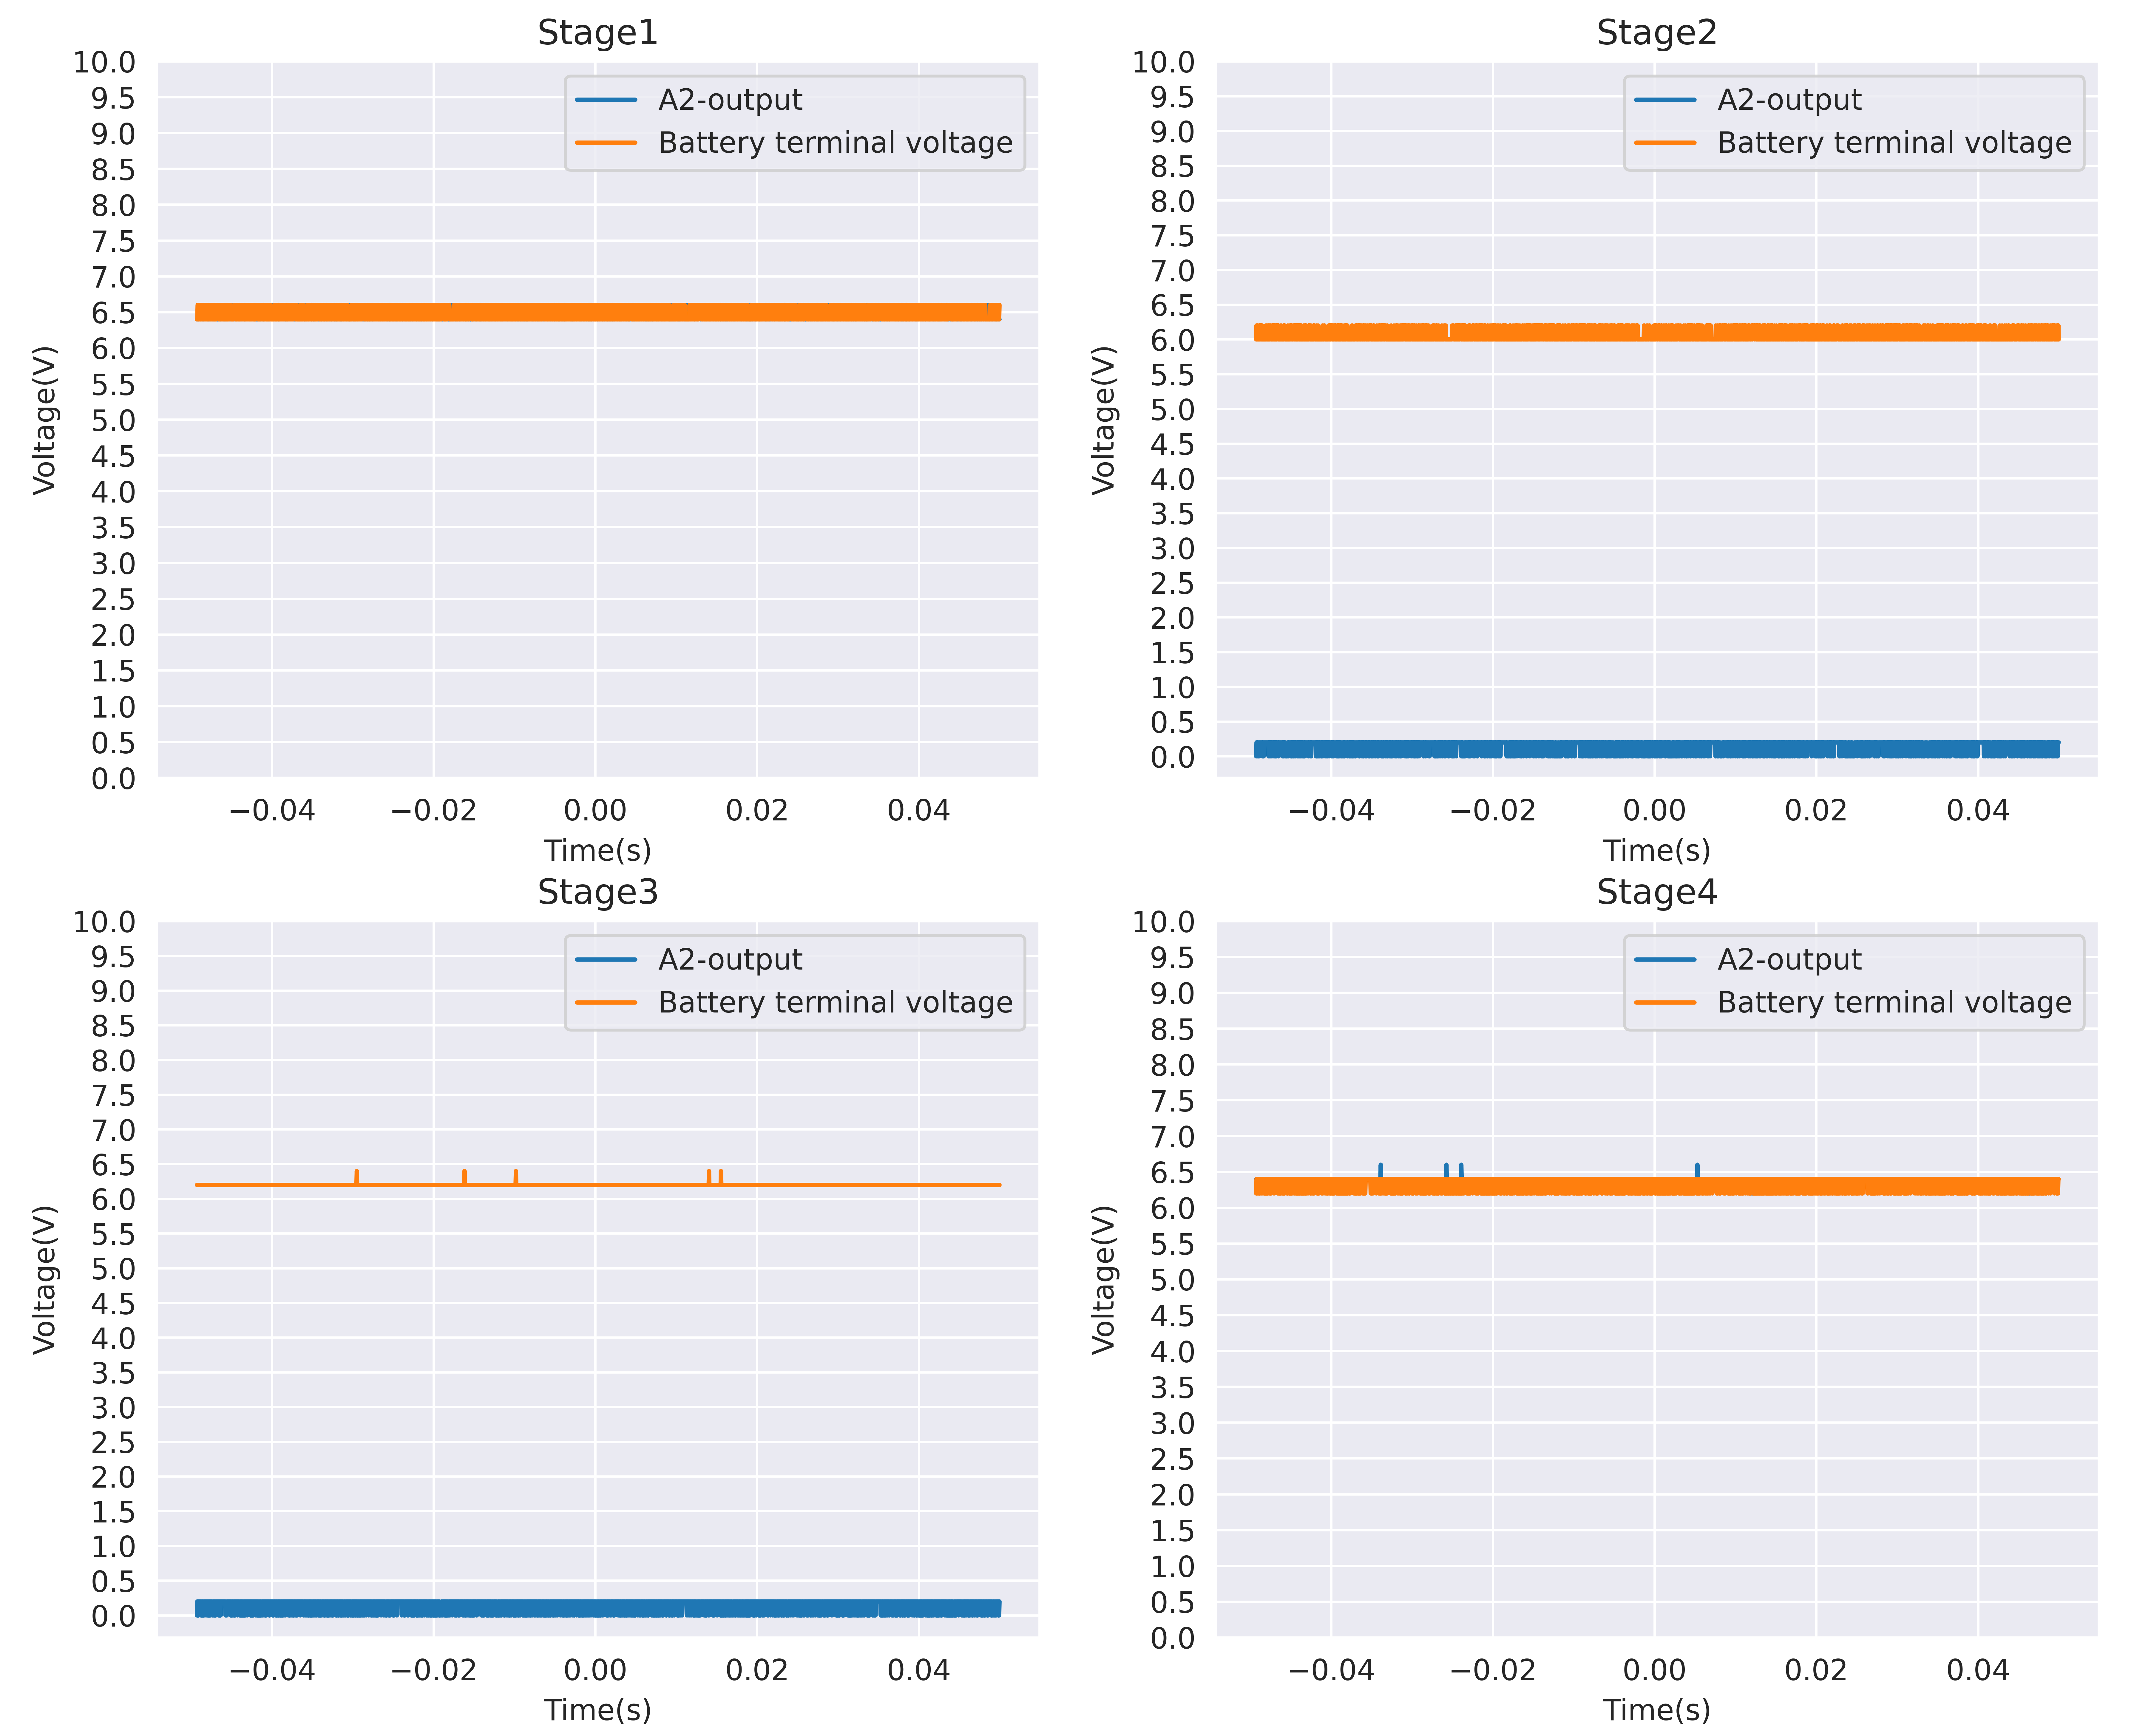
\includegraphics[scale=0.048]{./Figures/meas2.png}
\caption{Measured Oscilloscope results of under voltage circuit for 4 different stages of battery terminal voltages}
\label{fig:Oscil}
\end{figure}
\begin{flushleft}
\textbf{Stage 1}: Battery voltage is above 6V threshold and A2 output allows discharge.\newline
\textbf{Stage 2}: Battery voltage is below above 6V threshold and A2 output is 0V stopping battery discharge.\newline
\textbf{Stage 3}: Battery voltage is above 6V but not 6.2V (after under-voltage circuit disconnected battery) therefore A2 output is 0V, stopping battery discharge.\newline
\textbf{Stage 4}: Battery voltage is above 6.2V threshold after under-voltage circuit disconnected battery, therefore A2 is approximately equal to the battery voltage and is discharging.\newline
\end{flushleft}



%%%%%%%%%%%%%%%%%%%%%%%%%%%%%%%%%%%%%%%%%%%%%%%%%
\section{Current sense}


 \begin{figure}[!htb]
 \footnotesize
 \centering
    \begin{subfigure}[]{0.48\textwidth}
              \centering
  		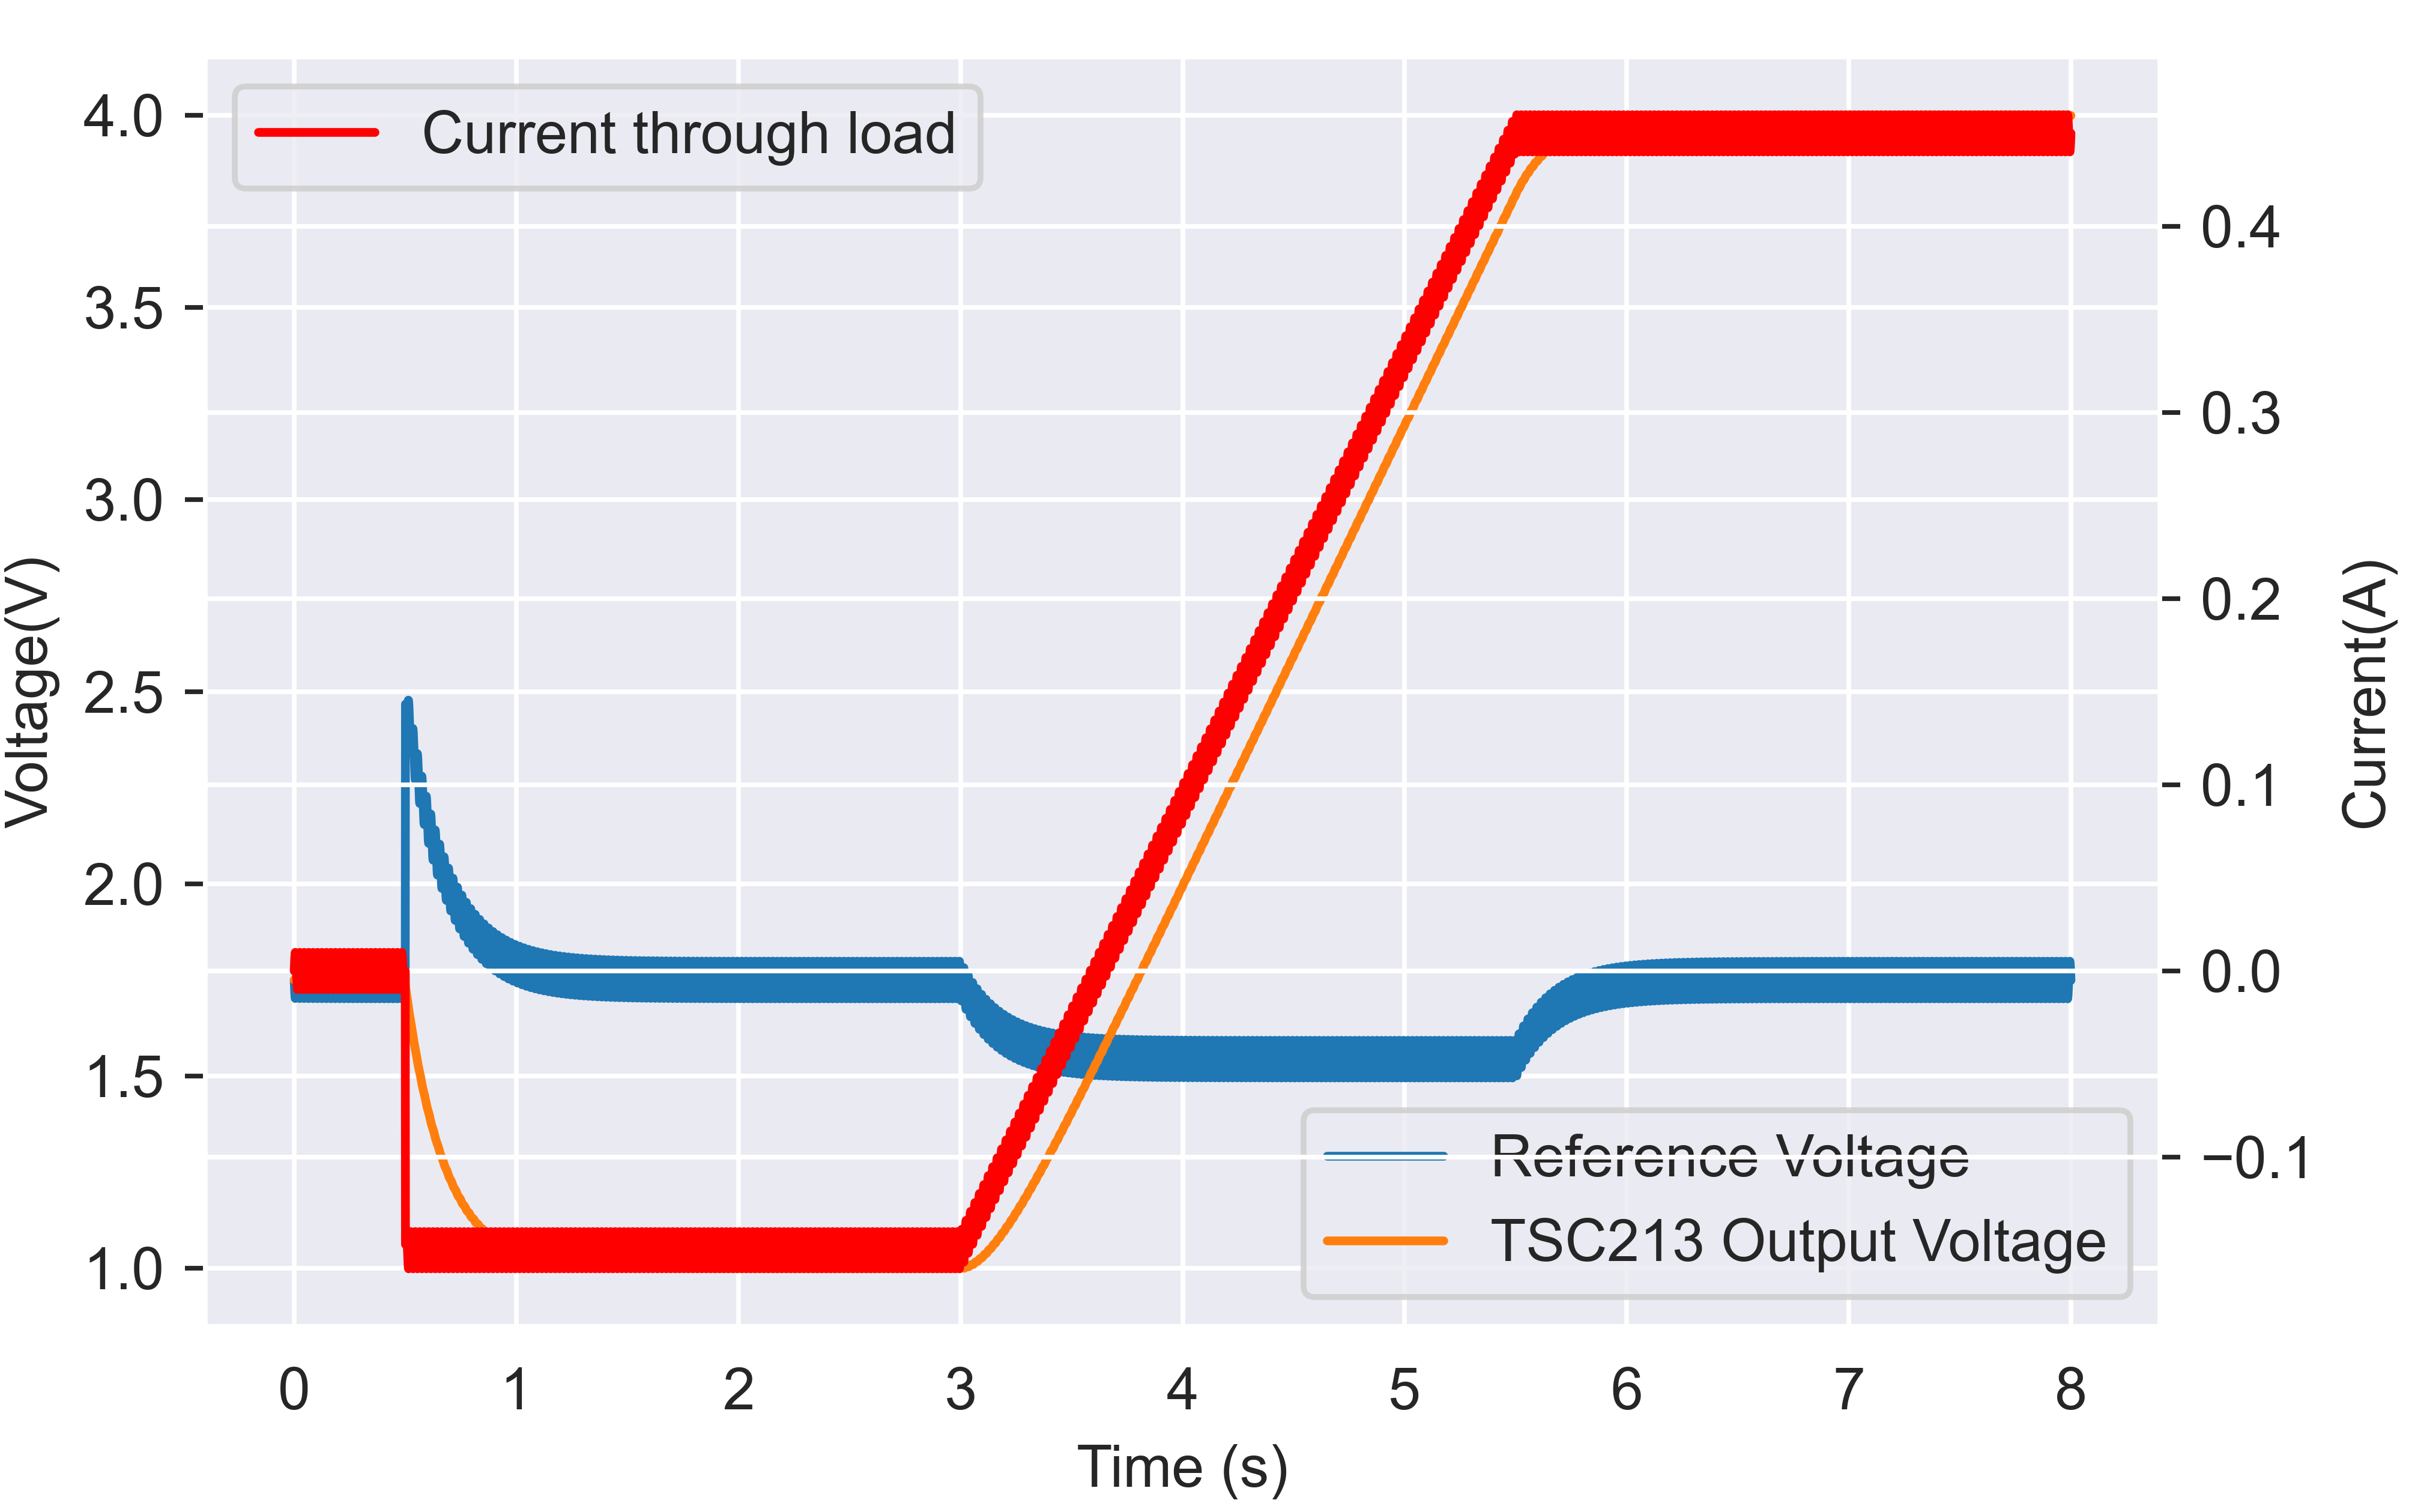
\includegraphics[width=1\linewidth]{./Figures/circuit.png}
		    \caption{} \label{subfig:sim}
     \end{subfigure}
     \begin{subfigure}[]{0.5\textwidth}
             \centering
  		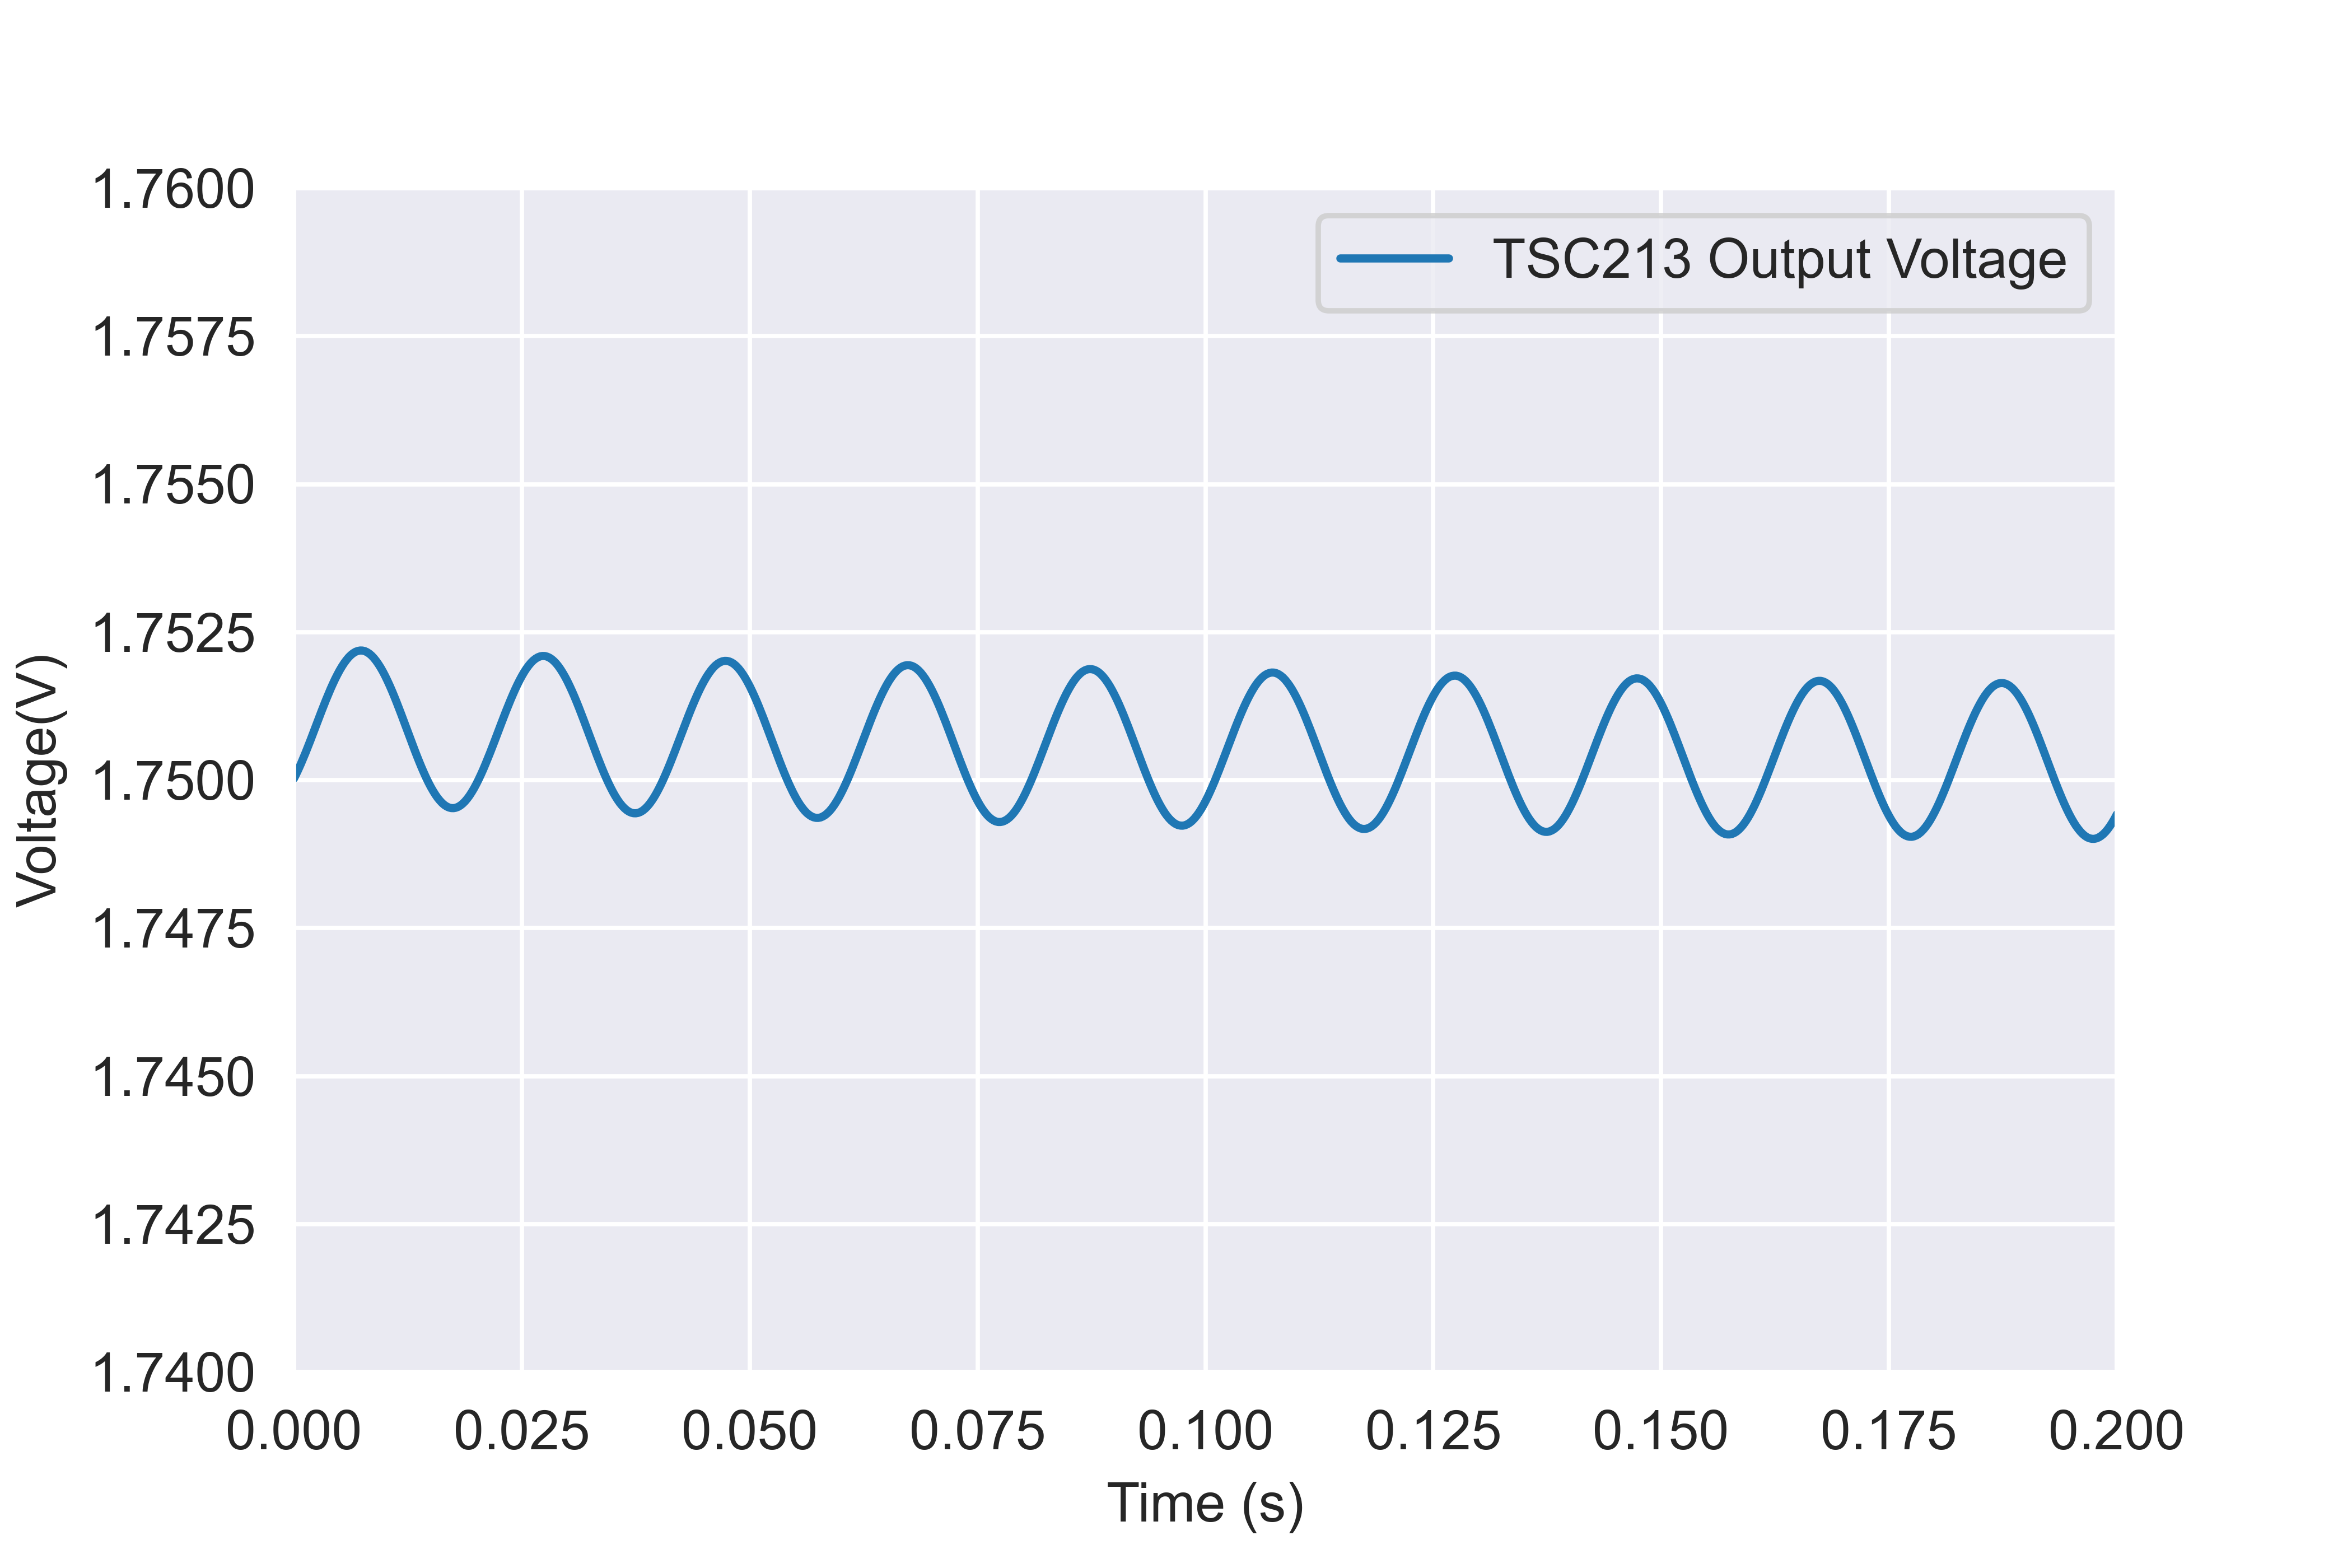
\includegraphics[width=1\linewidth]{./Figures/noise.png}
		   \caption{ } \label{subfig:noise}
     \end{subfigure}
   \caption[{Current Sense LTSpice Results}]{LT Spice results   (a)  Simulation results (b)Noise in output signal }
 
 \end{figure}

From figures \ref{subfig:noise} and \ref{subfig:sim} it can be seen that the necessary noise specifications are achieved and that the correct output range of 3V lies within the 0-5V boundary.
\begin{figure}[!htb]
\centering
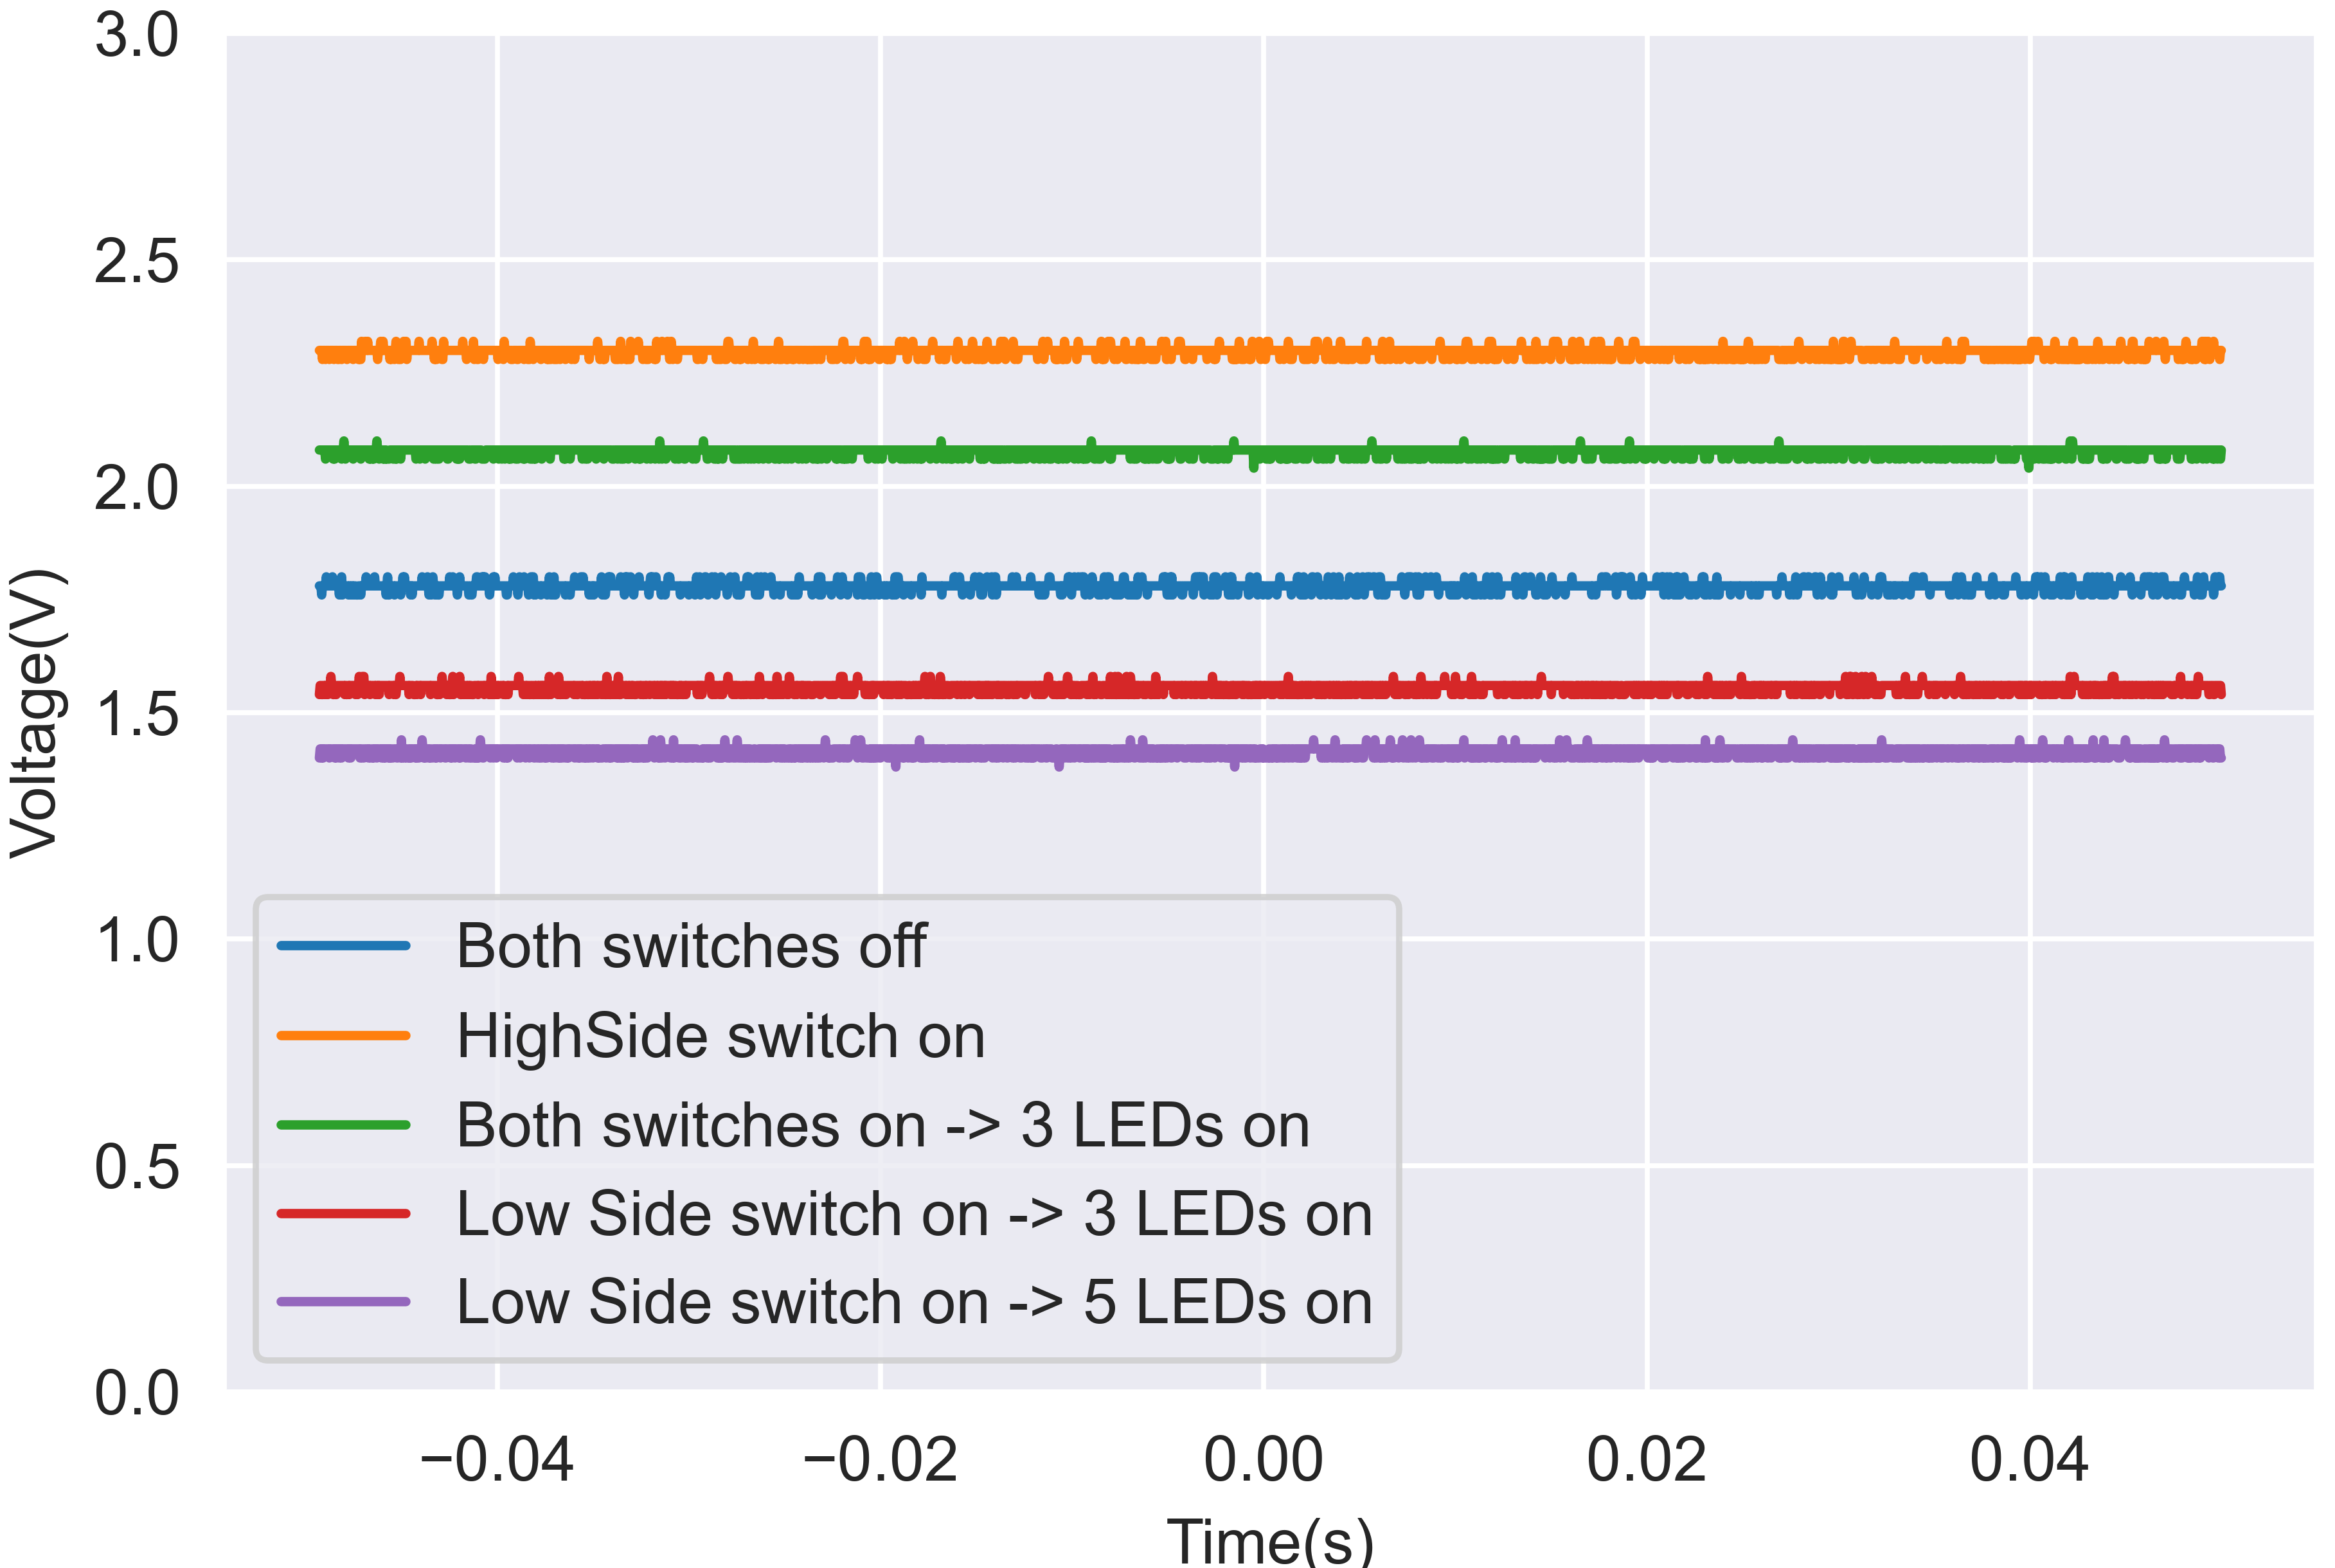
\includegraphics[scale=0.7]{./Figures/meas.png}
\caption{Oscilloscope measurements with various switch states}
\label{fig:meas}
\end{figure}

For the following explanation eq.\ref{eq:refeq} will help explain reasoning. When both switches are off the current flowing through the sense resistor is 0A as can be seen in figure \ref{fig:meas}.For this reason the output is equal to the reference voltage. When the High side switch turns on a positive current flows through the sense resistor, therefore the output increases. As the low side switch switches on, both switches are now on. The output voltage is still higher than the reference voltage because the charging current is greater than the discharging current resulting in a net positive current flow. When the high side switch then turns off the output voltage moves to below the reference voltage because now there is a net negative current through the resistor. As the last 2 LEDs are turned on the output of the TSC213 drops further as the negative (discharging) current increases.



\begin{table}[!htb]
        \centering
        \footnotesize
        \caption{Resistor measurements}
         \begin{tabular}{lrrrr}
          \toprule
             & $Resistor \ Voltage$ & $Calculated \ Current$ \\
             &  [V]  & [mA]\\
          \midrule
         R1      & 3.35 & 15.23 \\
          R2 & 3.34   & 15.18 \\
          R3       &3.36 & 15.27 \\
          R4        &3.35 & 15.23 \\
          R4        &3.37 &15.32 \\
          \bottomrule
        \end{tabular}
     \label{tab:resistor meas}
\end{table}



\begin{table}[!htb]
        \centering
        \footnotesize
        \caption{Measured results compared to actual results}
         \begin{tabular}{lrrrr}
          \toprule
             & TSC213 output voltage&Measured current flow & Indicated current flow& Error \\
             &   [V]&[mA]  &[mA]&[\%]\\
          \midrule
         Both switches off      & 1.75 &0 &0 &0 \\
         Low side switch on(3 LEDs)     & 1.525 & 45.8&45 &1.75 \\
         Low side switch on(5 LEDs)    & 1.383 & 73.4&76.2 &3.85 \\
          
          \bottomrule
        \end{tabular}
     \label{tab:compare}
\end{table}
The LT spice simulations(figure \ref{subfig:sim}) show the output working correctly and the noise( figure \ref{subfig:noise}) is within spec. The measured noise on the output of the TSC213 was found to be 40mV ($V_{PK-PK}$) on the oscilloscope. Larger capacitors were added to try reduce the noise, this was not successful. When the wall plug was powered off and only the battery was supplying the peak to peak voltage dropped to 8mV. This then identified the largest source of noise as the wall plug. Once again a large capacitor was used to try filter out the noise from the 12V, however this also did not decrease the output noise. The current through the LEDs is slightly less than 20mA as can be seen in table \ref{tab:resistor meas} as a result of the resistors chose in section \ref{sec:loadcontrol_design}. Regardless of the noise relatively accurate current measurements were obtained from the TSC213 output as can be seen in table \ref{tab:compare}.

%%%%%%%%%%%%%%%%%%%%%%%%%%%%%%%%%%%%%%%%%%%%%%%%%
\newpage
\section{Low-side switch}
\label{sec:loadcontrol_results}
 \begin{figure}[!htb]
 \footnotesize
 \centering
    \begin{subfigure}[]{0.42\textwidth}
              \centering
  		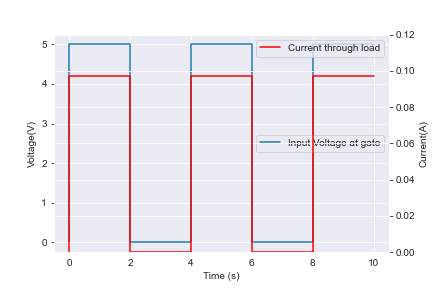
\includegraphics[width=1\linewidth]{./Figures/NMOS.png}
		    \caption{} \label{subfig:nmosfig}
     \end{subfigure}
     \begin{subfigure}[]{0.3\textwidth}
             \centering
  		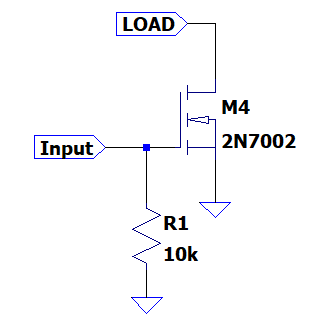
\includegraphics[width=1\linewidth]{./Figures/circNMOS.png}
		   \caption{ } \label{subfig:circnmos}
     \end{subfigure}
   \caption[{Fuse Characteristics}]{NMOS final Results   (a)  LT Spice simulation (b)Lowside circuit used }
    \label{fig:NMOScirc}
 \end{figure}
 The above LTspice simulation in figure \ref{subfig:nmosfig} was setup to have a load that had 100mA flowing through it. It shows that the NMOS was able to switch this amount of current with ease using a 5V control signal. Using this circuit practically the low side switching in figure \ref{fig:meas} was achieved, indicating that it was able to enable and disable discharge through the load.


\begin{figure}[!htb]
\centering
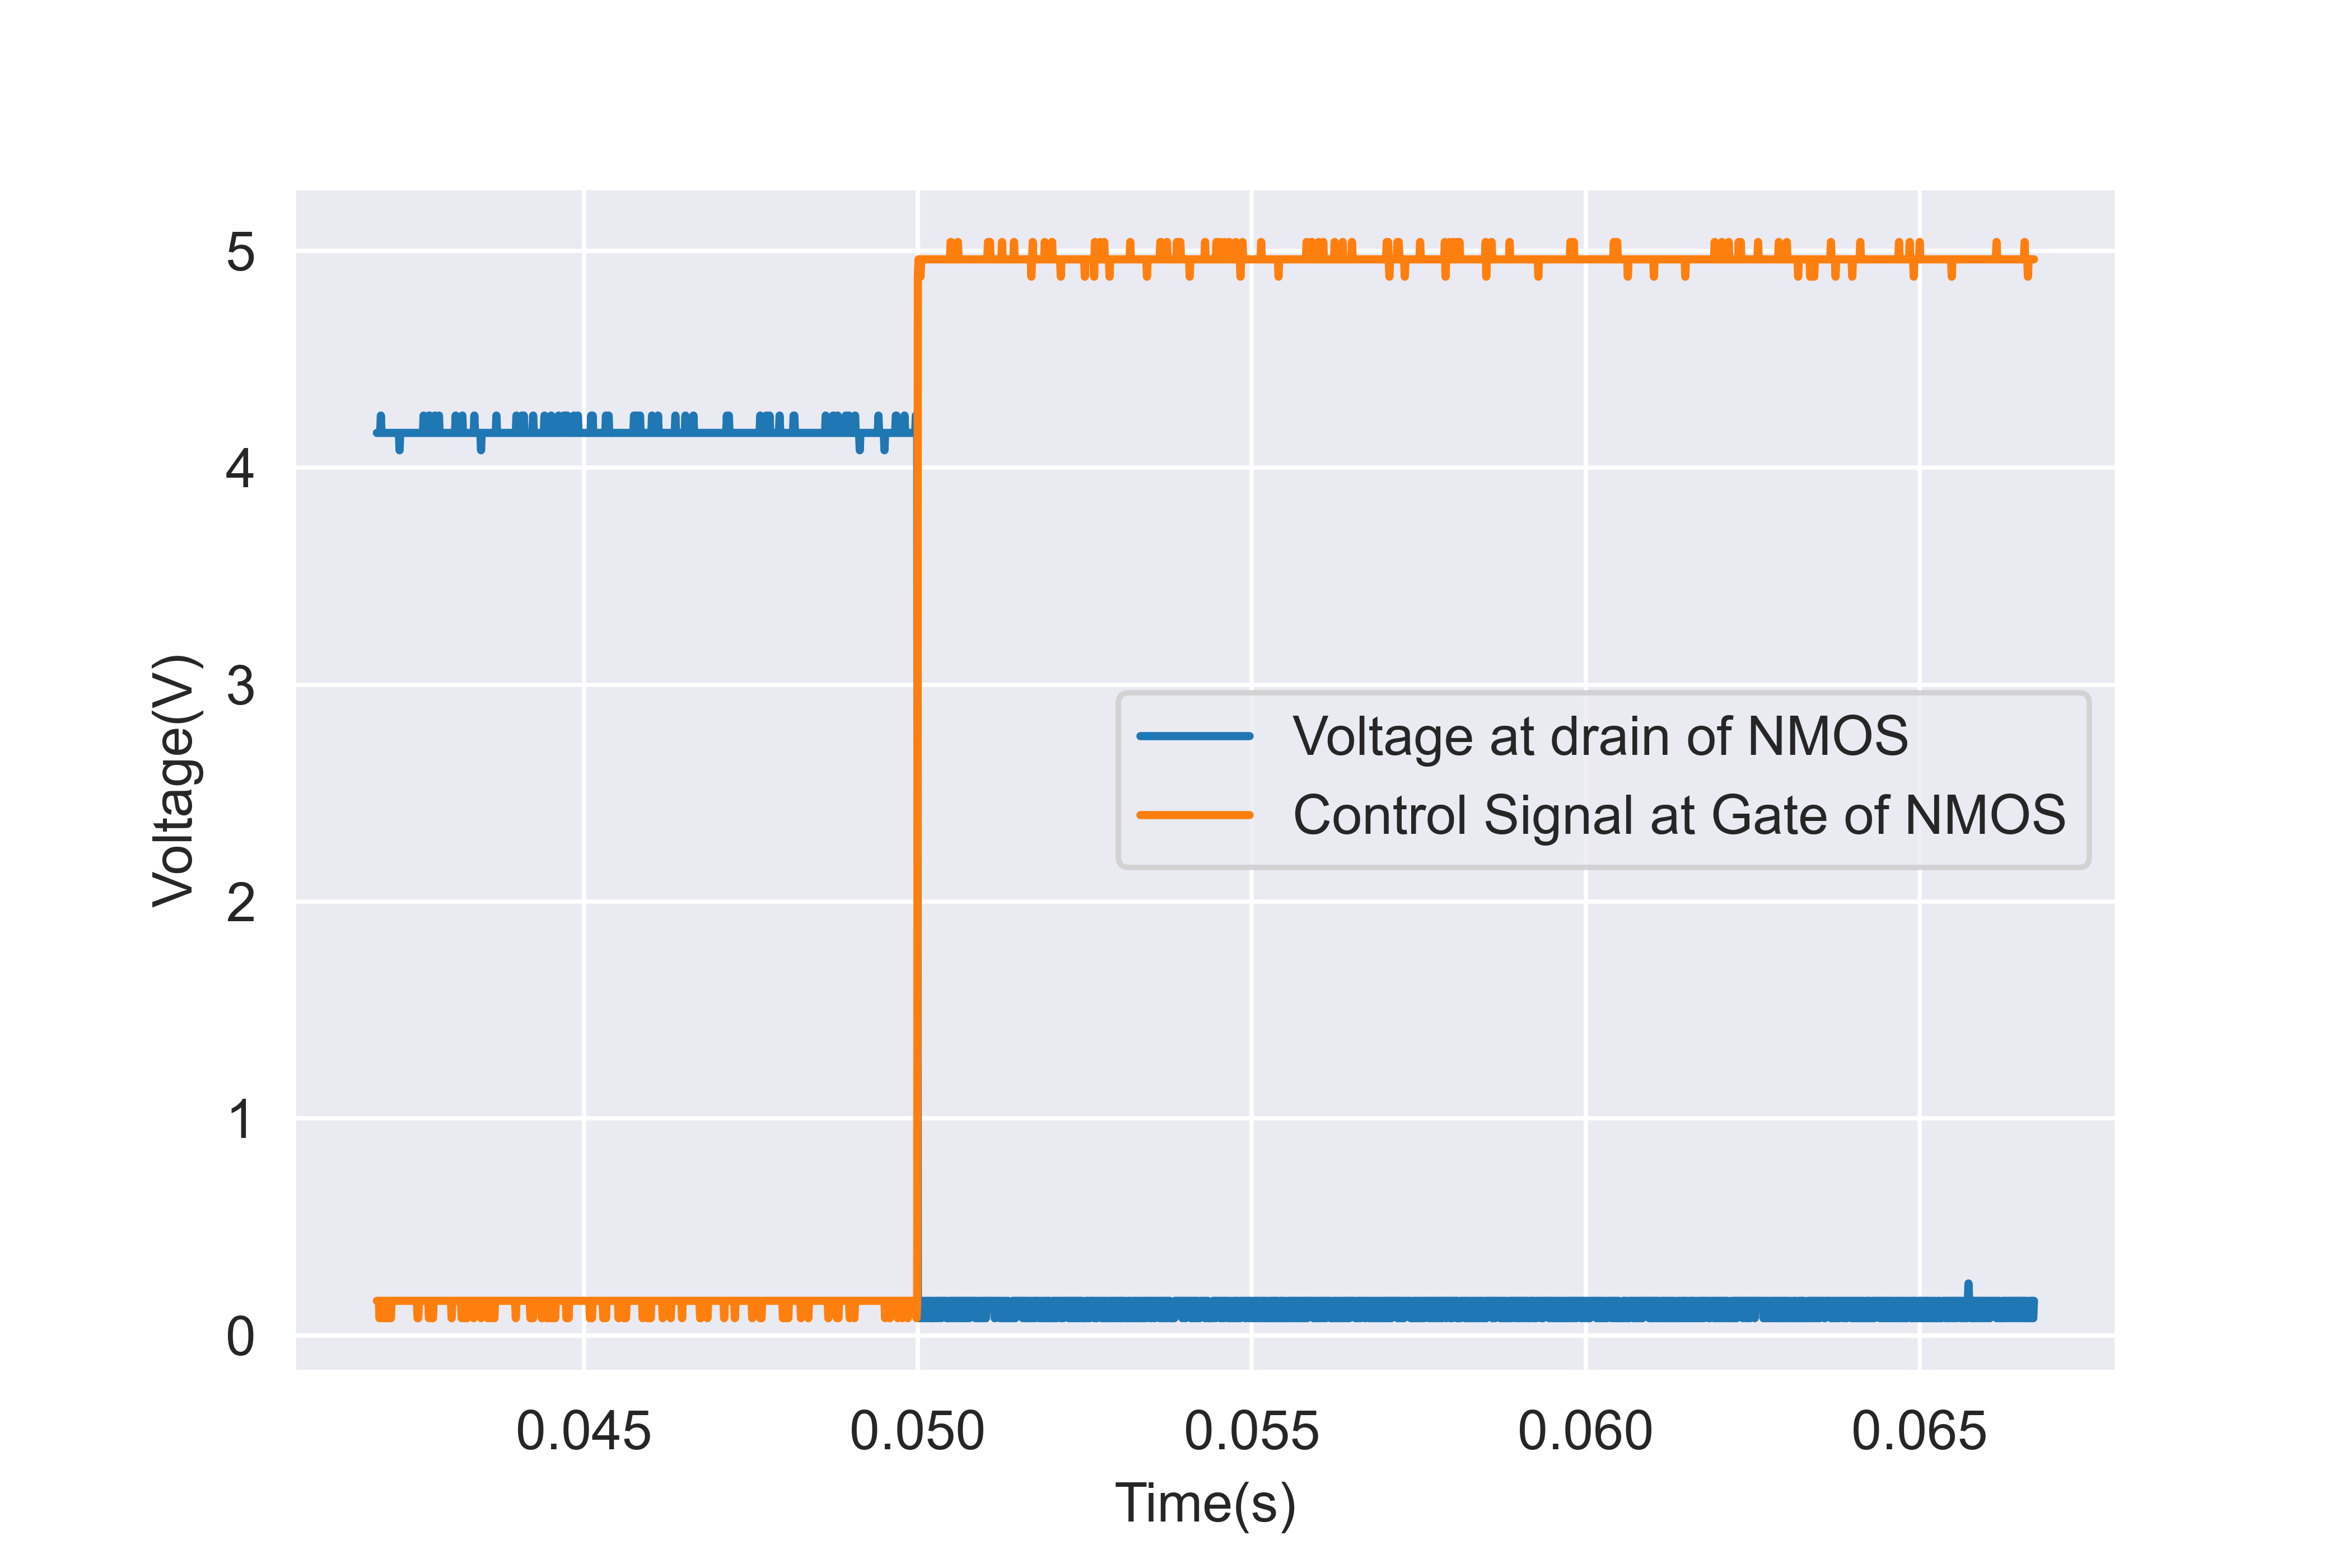
\includegraphics[scale=0.6]{./Figures/NMOSmeas}
\caption{Oscilloscope Measurements of NMOS while switching}
\label{fig:measNMOS}
\end{figure}

From figure \ref{fig:measNMOS} it can be seen that the switching time of the NMOS is virtually instantaneous and also simply that the NMOS switching capability is working correctly. The NMOS source is connected to ground, therefore when the control signal goes high the NMOS "connects" its drain to its source which is ground.

%%%%%%%%%%%%%%%%%%%%%
